%% эта глава концептуально соответсствует предпоследнему слайду моей презентации
%% Universal EDM measurement problems
%% where I have two categories of problems: those solved by using a Spin Wheel,
%% and those having specific solutions
%% the SMP section here covers the SW-solvable problems: stray fields and betatron motion
%% then Spin decoherence and machine imperfections are considered specifically


\chapter{Общие проблемы методов поиска ЭДМ в накопительном кольце, и их решения} \label{chpt3:top-level}
 
Универсальные проблемы методов по поиску ЭДМ фундаментальных частиц в накопительном кольце можно разделить на 
две категории:
\begin{enumerate*}[\itshape i\upshape)]
	\item проблемы, решаемые введением в систему Спин-Колеса, и
	\item проблемы, имеющие специфические решения.
\end{enumerate*}

Проблемы первой категории следуют из нестабильности оси стабильного спина частиц. К ним относятся, например, 
локальные возмущения электромагнитных полей, а также бетатронные колебания частиц. В обоих случаях, ось стабильного спина частицы отклоняется от своего равновесного значения на непродолжительное время.

К проблемам, имеющим специфические решения относятся спин-декогеренция, и фальш-сигнал, вызванный 
неидеальностями ускорителя. В этом разделе мы рассмотрим суть каждой из данных проблем, опишем их возможные
решения, и проведём соответствующие симуляции.
  
\section{Возмущения спиновой динамики}\label{chpt3:smp}
\documentclass[a4paper]{jacow}
\usepackage{mathtools}
\usepackage{amsmath}
\usepackage{xfrac}
\usepackage{xparse}
\usepackage{subcaption}
\usepackage{graphicx}
\usepackage{url}
\usepackage{paralist}
\usepackage{multirow}
\usepackage{siunitx}

\let\oldvec\vec
\renewcommand{\vec}{\boldsymbol}
\DeclareDocumentCommand{\bkt}{sm}{\IfBooleanTF{#1}{\left[ #2 \right]}{\left(#2\right)}}
\DeclareDocumentCommand{\ddt}{m}{\frac{\mathrm{d} {#1}}{\mathrm{d} t}}
\DeclareDocumentCommand{\pddx}{mO{t}O{}}{\frac{\partial^{#3} {#1}}{\partial {#2}^{#3}}}
\newcommand{\w}{\omega}
\newcommand{\W}{\Omega}
\newcommand{\avg}[1]{\langle {#1} \rangle}
\newcommand{\nbar}{\bar n}


\begin{document}
\title{Spin Motion Perturbation Effect on the EDM Statistic in the Frequency Domain Method}
\author{A. E. Aksentyev\textsuperscript{1}\thanks{alexaksentyev@gmail.com},
  Institut f\"ur Kernphysik, Forschungszentrum J\"ulich, J\"ulich, Germany \\
  Y. V. Senichev, Institute for Nuclear Research of RAS \\
  \textsuperscript{1}also at National Research Nuclear University ``MEPhI,'' Moscow, Russia}
\maketitle
\footnotetext[2]{a.aksentev@fz-juelich.de}
\begin{abstract}
  The spin precession axis of a particle involved in betatron motion precesses about the invariant spin axis
  defined on the closed orbit (CO). This precession can be observed in polarization data as a rapid,
  small-amplitude oscillation on top of the major effect oscillation caused by the precession of spin
  about the CO axis. The frequency of this latter oscillation is used in the Frequency Domain methodology
  as the EDM observable. It is estimated by fitting polarimetry data by a sine function; the rapid
  oscillations, therefore, constitute a model specification error.
  This model error will introduce a bias into the frequency estimate. In the present work we investigate
  how this bias changes depending on the beam revolution direction, its stability over time, and
  the EDM estimate error introduced by it.
\end{abstract}

\section{Frequency Domain methodology}
Frequency Domain (FD)~\cite{Senichev:FDM} is a Storage Ring method of search for the
Electric Dipole Moment (EDM) of a fundamental particle.~\cite{BNL:SREDM}
It belongs to the Frozen Spin~\cite{BNL:Deuteron2008} category
of such methods, i.e., the Magnetic Dipole Moment (MDM) component of spin precession is minimized. However,
the original Frozen Spin method proposed in~\cite{BNL:Deuteron2008} is a Space Domain
method~\cite[p.~4]{Talman:ElectricRings}: inferences about the EDM are drawn from the change of orientation
of the polarization vector, as measured by the angle between its initial and final orientations. This approach
has the following problems:
\begin{inparaenum}[\itshape a\upshape)]
\item it puts very stringent constraints on the precision of the accelerator optical element alignment, and
\item it poses a challenging task for polarimetry.~\cite[p.~6]{Mane:SpinWheel}
\end{inparaenum}

The former is to minimize the magnitude of
the vertical plane MDM precession frequency:~\cite[p.~11]{BNL:Deuteron2008}
\begin{equation}\label{eq:BNL_syst_err}
\w_{syst} \approx \frac{\mu\avg{E_v}}{\beta c\gamma^2},
\end{equation}
induced by field imperfections. The latter is due to the requirement of detecting a change of about
$5\cdot 10^{-6}$ to the cross section $\varepsilon_{LR}$ in order to get to the EDM sensitivity level
of $10^{-29}~e\cdot cm$.~\cite[p.~18]{BNL:Deuteron2008}

EDM search methods in the Frequency Domain circumvent the above problems: EDM inferences are based
on the rate of change of the aforementioned polarization orientation angle. The polarization vector is made to
roll about a nearly-constant, definite direction vector $\nbar$, with an angular velocity
that is large enough for the beam polarization to be easily measureable at all times. This ``Spin Wheel'' may be
externally applied~\cite{Koop:SW}, or otherwise the machine imperfection fields
may be utilized for the same purpose~\eqref{eq:BNL_syst_err}~\cite{Senichev:FDM}. The latter is made possible
by the fact that $\w_{syst}$ changes sign when the beam revolution direction
is reversed.~\cite[p.~11]{BNL:Deuteron2008}

The frequency of oscillation of the vertical polarization component $P_y$ is estimated
via a fit of the polarimetry data to the model
\begin{equation}\label{eq:fit_model}
  f(t) = a\cdot\sin(\w\cdot t + \delta).
\end{equation}

\section{Problem statement}
\newcommand{\ntrn}{n_{turn}}
Consider the case of a single particle beam. The solution of the T-BMT equation for the
vertical spin-vector component has the general form
\begin{equation}\label{eq:sy_growth_1}
  s_y(t) = \sqrt{\bkt{\frac{\w_y\w_z}{\w^2}}^2 + \bkt{\frac{\w_x}{\w}}^2}\cdot\sin\bkt{\w\cdot t + \delta},
\end{equation}
where $\vec\w = (\w_x, \w_y, \w_z)$ is a function of time as a result of betatron motion.

Using $\vec\w = 2\pi f_{rev}\nu_s\nbar$~\cite[p.~4]{COSY:SpinTuneMapping}, equation~\eqref{eq:sy_growth_1}
can be reformulated in terms of spin tune $\nu_s$ and invariant spin axis $\bar n$:
\begin{equation}\label{eq:main}
  s_y(n_{turn}) = \sqrt{\bkt{\nbar_y\nbar_z}^2 + \nbar_x^2}\cdot\sin\bkt{2\pi\nu_s\cdot\ntrn + \delta},
\end{equation}
where $\nbar = \nbar(\ntrn)$ and $\nu_s = \nu_s(\ntrn)$ are functions of the turn number $\ntrn$.

Sufficiently large variation of~ $\nbar$ and/or $\nu_s$ can lead to model specification systematic error.
Variation in $\nu_s$ is especialy problematic in this regard, as it directly affects the phase of the signal;
however, this problem can be solved by the introduction of sextupole fields into the system,
as described in~\cite{Aksentev:DecohIPAC19}. In this paper we will, therefore, be concerned only with the $\nbar$
variation.

\section{Simulation}
The simulation setup was as follows: a particle, offset from the design orbit in the vertical
direction by 0.3 mm, is injected multiple times into an imperfect
Frozen Spin lattice~\cite{Senichev:Lattices} utilizing sextupoles for
the reduction of spin decoherence caused by vertical plane betatron
oscillations~\cite{Aksentev:DecohIPAC19}. Lattice imperfections are simulated by rotations of the E+B spin
rotator elements. Imperfections introduced this way do not perturb the design orbit.

Each injection, the rotation angles are randomly generated from the
normal distribution $\alpha\sim N(\mu_i, 3\cdot 10^{-4})$ degrees, $i\in\{1,\dots,41\}$, where
$\mu_i$ varies in the range $[-1.5\cdot10^{-4}, +2.5\cdot10^{-4}]$ degrees. The non-zero expectation values $\mu_i$
simulate the application of a Koop Spin Wheel (SW).~\cite{Koop:SW} The magnitudes of $\mu_i$ and $\sigma_{\alpha}$
are chosen for effect detalization purposes.

Another aspect of the simulation worth noting, is that injection occurs at 270 MeV, while the FS condition
is fullfilled exactly at 270.0092 MeV. Because of that the invariant spin axis $\nbar$
points mainly in the vertical direction (deviating from it by no more than \ang{51} at higher SW roll speeds);
its radial component (the one determining the oscillation amplitude of the vertical spin-vector component)
is relatively small, and all the more susceptible to variation caused by vertical plane betatron motion for that. 

Spin tracking is done in COSY Infinity~\cite{COSYINF:Website}, for $1.2\cdot10^6$ turns; each 800 turns
$\nu_s$ and $\nbar$ are computed (by means of procedure TSS~\cite[p.~41]{COSYINF:BeamPhysMan}) at
the phase space point occupied by the particle at the time, giving us the series $(\nu_s(n), \nbar(n))$.
The corresponding spin vector components $(s_x^{trk}(n), s_y^{trk}(n), s_z^{trk}(n))$,
computed by the tracker (procedure
TR~\cite[p.~41]{COSYINF:BeamPhysMan}), 
constitute the second series used in the analysis.

\section{Analysis}
Using the first series data, we generated the expected $s_y^{gen}(t)$ ``generator'' series according to
equation~\eqref{eq:main}, as well as the ``ideal'' series $s_y^{idl}$, in which
we assumed constant values of $\nu_s = \avg{\nu_s(t)}$ and $\nbar
=\avg{\nbar(t)}$. 

Our hypothesis is that the particle's betatron
motion should introduce a mismatch between the sinusoidal
model~\eqref{eq:fit_model} and tracker data, by varying the direction
of the spin precession axis $\nbar$, and hence the amplitude of the
fitted signal. The ``ideal'' series serves as the baseline of our
analysis, as it's a perfect match to the model; the ``generator''
series incorporates $\nbar$ variation, still remaining within the confines of
the model. The ``tracker'' series is the closest approximation to
real measurement data.

To compare these series with one another, we
\begin{inparaenum}[\itshape a\upshape)]
\item computed and analyzed the residuals
  $\epsilon_1(t) = s_y^{gen}(t) - s_y^{idl}(t)$, and
  $\epsilon_2(t) = s_y^{trk}(t) - s_y^{idl}(t)$;
\item fitted model~\eqref{eq:fit_model} to the three time series and
  compared its goodness-of-fit;
\item computed the standard deviations of $\nbar$ components at each
  spin wheel strength.
\end{inparaenum}

\begin{figure}[h]
  \centering
    \includegraphics[width=\linewidth]{../img/IPAC19/residual_vs_time(both)}
  \caption{Time series' comparator residual as a function of time.
    Top panel: residual $\epsilon_1$; bottom panel: residual $\epsilon_2$\label{fig:residuals}}
\end{figure}

\begin{figure}[h]
  \centering
  \begin{subfigure}{\linewidth}
    \centering
    \includegraphics[width=\linewidth]{../img/IPAC19/NBAR_variation_sd_vs_SW}
    \caption{Of the $\nbar$ components\label{fig:sd:nbar}}
  \end{subfigure}
  \begin{subfigure}{\linewidth}
    \centering
    \includegraphics[width=\linewidth]{../img/IPAC19/residual_SD_vs_SW(both)}
    \caption{Of the comparator residuals.
      Top panel: residual $\epsilon_1$; bottom panel: residual $\epsilon_2$\label{fig:sd:res}}
  \end{subfigure}
  \caption{Standard deviations versus relative Spin Wheel strength\label{fig:sd}}
\end{figure}

\begin{table}[h]
  \caption{Model parameter estimates (slowest SW roll)\label{tbl:param_estimates}}
  \begin{tabular}{r|rllr}
    \toprule
    Data & Par. & Value & St.Error & AIC \\
    \midrule
    \multirow{3}{*}{$s_y^{idl}$}
    & $\hat f$ & 4.220359687911 & $6.9\cdot 10^{-11}$ & \multirow{3}{*}{-62093} \\
    & $\hat a$ & 0.12514597851 & $4\cdot 10^{-11}$ & \\
    & $\hat\delta$ & $-1.50\cdot 10^{-8}$ & $4\cdot 10^{-10}$ &\\
    \hline
    \multirow{3}{*}{$s_y^{gen}$}
    & $\hat f$ & 4.2203596911 & $1.9\cdot 10^{-9}$ & \multirow{3}{*}{-52142} \\
    & $\hat a$ & 0.125145979 & $1\cdot 10^{-9}$ & \\
    & $\hat\delta$ & $-1.6\cdot 10^{-8}$ & $1.2\cdot 10^{-8}$ &\\
    \hline
    \multirow{3}{*}{$s_y^{trk}$}
    & $\hat f$ & 4.2203603 & $1.3\cdot 10^{-6}$ & \multirow{3}{*}{-34567} \\
    & $\hat a$ & 0.12514597 & $3.7\cdot 10^{-7}$ & \\
    & $\hat\delta$ & $-4\cdot 10^{-6}$ & $6\cdot 10^{-6}$ &\\
    \bottomrule
  \end{tabular}
\end{table}

What we observe in Figure~\ref{fig:residuals} is that the ``generator'' series is nearly identical
to the ``ideal'' series (even if its frequency is slightly different), with $\epsilon_1 \le 1\cdot10^{-6}$
during run time,
while the ``tracker'' series deviates from it at the level
$\epsilon_2 \le 2\cdot 10^{-5}$. This discrepancy between $\epsilon_1$ and $\epsilon_2$ is observed
systematically across all spin wheel strengths (cf. Figure~\ref{fig:sd:res}), and has no explanation as of yet.

In Figure~\ref{fig:sd:res} we see that the standard deviations of both residuals exhibit the same pattern as
the standard deviation of $\nu_s$ (Figure~\ref{fig:sd:nbar}, bottom panel), but not as that of
the $\nbar$ components. This is an indication that frequency variation is a much more significant factor
in the mismatch between model~\eqref{eq:fit_model} and tracker data, than is the presumed amplitude variation
due to the change of orientation of $\nbar$.

Table~\ref{tbl:param_estimates} characterizes the fit model's goodness-of-fit with respect to the time series,
in the case of the slowest-rolling Koop Wheel.
One observes that the differences between the parameter estimates of all three series are not
statistically significant. Even though variation of the spin precession angular velocity vector worsened
the fit quality of the model, it didn't introduce any statistically-significant bias
into the estimates.

\section{Conclusions}
The question of the influence of betatron motion on the EDM statistic in the FD method should be considered
in view of three circumstances:
\begin{enumerate}
\item The signal amplitude oscillations (as estimated by $\epsilon_2$) are small.
  They occur at the $10^{-4}$ level (when $\sigma_{\alpha}=5\cdot 10^{-4}$), whereas
  the expected polarization measurement error is on the order of percents.
  This means the superposition of this systematic error with the random measurement error
  will exhibit no statistically-significant systematicity.
\item The correllation coefficient between the amplitude and frequency estimates is not significant. The amplitude
  oscillations affect the $\hat a$-estimate foremost; their effect on the $\hat\w$-estimate is secondary, and is
  described by the correlation coefficient. Since it is less than 10\%, even if the oscillations happen to be
  strong enough to affect the amplitude estimate, their effect on the frequency estimate will be reduced by
  at least a factor of 10.
\item This systematic effect is controllable. And this point is the major advantage of the FD methodology.
  By applying an external Spin Wheel, the $\nbar$ oscillations can be continuously minimized
  as much as necessary, without changing the experiment pattern.
\end{enumerate}

\begin{thebibliography}{9}

\bibitem{Senichev:FDM}
  Y. Senichev, A. Aksentev, A. Ivanov, E. Valetov, ``Frequency domain method of the search for
  the deuteron electric dipole moment in a storage ring with imperfections,'' arxiv:1711.06512 [physics.acc-ph]
  \url{https://arxiv.org/abs/1711.06512}.

\bibitem{BNL:SREDM}
  M. Bai et al., SREDM Collaboration website: \url{https://www.bnl.gov/edm/}.

\bibitem{BNL:Deuteron2008}
  D. Anastassopoulos et at., (srEDM Collaboration), ``Search for a permanent electric dipole moment of
  the deuteron nucleus at the $10^{-29}~e\cdot cm$ level,'' proposal as submitted to the BNL PAC, April 2008.

\bibitem{Talman:ElectricRings}
  R. Talman, ``Prospects for Electric Dipole Moment Measurement Using Electrostatic Accelerators,''
  Reviews of Accelerator Science and Technology, A. Chao and W. Chou, editors, Volume 10, 2018, not yet in print.

\bibitem{Mane:SpinWheel}
  S. Mane, ``A distillation of Koop's idea of the Spin Wheel,'' arXiv:1509.01167 [physics]
  \url{http://arxiv.org/abs/1509.01167}.

\bibitem{Koop:SW}
  I. Koop. ``Asymmetric energy colliding ion beams in the EDM storage ring,'' Proc. of IPAC13 (2013).
  \url{http://accelconf.web.cern.ch/accelconf/ipac2013/papers/tupwo040.pdf}.

\bibitem{COSY:SpinTuneMapping}
  A. Saleev et al., (JEDI Collaboration), ``Spin tune mapping as a novel tool to probe
  the spin dynamics in storage rings.'' Phys. Rev. Accel. Beams 20 (2017) no.7, 072801.

\bibitem{Aksentev:DecohIPAC19}
  A. Aksentev, Y. Senichev, ``Spin decoherence in the Frequency Domain Method for the search of a particle EDM,''
  presented at the 10th International Particle Accelerator Conf. (IPAC’19), Melbourne, Australia,
  May. 2019, paper 2738, this conference.

\bibitem{Senichev:Lattices}
  Y. Senichev, S. Andrianov, S. Chekmenev, M. Berz, E.Valetov. ``Investigation of Lattice for Deuteron EDM Ring,''
  Proc. of ICAP15 (2015). \url{http://accelconf.web.cern.ch/AccelConf/ICAP2015/papers/modbc4.pdf}.

\bibitem{COSYINF:Website}
  M. Berz, K. Makino, COSY Infinity website: \url{cosyinfinity.org}.

\bibitem{COSYINF:BeamPhysMan}
  M. Berz, K. Makino. COSY INFINITY 10.0 Beam Physics Manual.

\end{thebibliography} 
\end{document}


\section{Декогеренция спинов частиц пучка}\label{chpt3:decoherence}
Когеренцией спина называется мера или качество сохранения поляризации
в изначально полностью поляризованном пучке.~\cite[стр.~205]{Eremey:Thesis}

Когда поляризованный пучок инжектируется в накопительное кольцо, спин-векторы 
частиц пучка начинают прецессировать вокруг вертикального
(ведущего) поля. Частота прецессии зависит от равновесного уровня
энергии частицы, который различен для частиц пучка.

Это обстоятельство не является проблемой в том случае, когда начальная
поляризация пучка вертикальна; однако метод измерения ЭДМ в
накопительном кольце, основанный
на принципе замороженного спина требует, чтобы вектор поляризации
пучка был сонаправлен с его вектором импульса, т.е. лежал в
горизонтальной плоскости. Таким образом, декогеренция спина есть
внутренняя проблема метода замороженного спина.

В настоящем разделе мы исследуем причины возникновения спин-декогеренции,
метод борьбы с ней, а также приведём результаты симуляции, подтверждающей действенность
метода. Для начала, однако, определим время когеренции спина, требуемое для 
измерения ЭДМ методом замороженного кольца в пространственной области.



\subsection{Spin coherence time requirements}
Operating in the space domain FS methodological framework in a perfectly-aligned lattice,~\footnote{In fact,
perfect element alignment is a pre-requirement of the space domain.}
the spin coherence time (SCT) is determined by the minimal detectable angle
by which the polarization vector deviates from the beam orbit plane as a result of the EDM action
alone. For the sensitivity level of $10^{-29}~e\cdot cm$ this angle is approximately
$5\cdot10^{-6}$.~\cite{BNL:Deuteron2008}

According to the T-BMT equation,
\[
\W_{EDM,x} = \eta\frac{qE_x}{2mc},
\]
where $\eta$ is the proportionality coefficient between the EDM and spin,
in the deuteron case equal to $10^{-15}$, for the given sensitivity level.~\cite[p.~206]{Eremey:Thesis}

For the deuteron BNL FS ring, $E_x = 12$
MV/m,~\cite[p.~19]{BNL:Deuteron2008} therefore $\W_{EDM,x}\approx 10^{-9}$ rad/sec.
Hence we obtain that, in order to reach a detectable level of at least 1 $\mu$rad one needs an SCT
on the order of 1,000 seconds.~\cite[p.~207]{Eremey:Thesis}
\subsection{Origins of decoherence}\label{sec:decoh:origin}
Spin decoherence in a particle beam results from the dispersion of the beam particles'
spin precession angular velocities, which, in its turn, is a result of the difference
between their orbit lengths and initioal momenta. The orbit length effect on the particle spin tune
is described by the concept of the effective Lorentz-facotr, which was introduced
in section~\ref{chpt1:FS-methods:effective-Lorentz-factor}.

Frim equations~\eqref{eq:spin_tune_vs_gamma} for spin tune in electrostatic and magnetic fields it follows that 
the spin tunes of two particles having equal values of the effectove L-factor are equal, regardless of
their trajectories in the accelerator. This principle is the basis for the proposed sextupole field
spin precession suppression theory, as well as the procedure for flipping the polarity of the storage ring's
guide field, which is required for injecting the deuteron beam in the opposite direction in order to cancel
the EDM-faking MDM spin precession.

\subsection{Sextupole field spin decoherence suppression theory}\label{sec:sextupole_spin_dec_solution}
In order to minimize spin decoherence related to particle betatron motion and momentum spread
sextupole (or octupole) fields can be used.~\cite[p.~212]{Eremey:Thesis}

A sextupole of strength
\[
S_{sext} = \frac{1}{B\rho} \pddx{B_y}[x][2],
\]
where $B\rho$ is the magnetic rigidity, modifies the first-order momentum
compaction factor as~\cite[p.~2581]{Senichev:IPAC13}
\begin{align}
	\Delta \alpha_{1,sext} &= -\frac{S_{sext}D_0^3}{L}, \label{eq:Sext_compaction_effect}
	\intertext{and simultaneously the orbit length as}
	\bkt{\frac{\Delta L}{L}}_{sext} &= \mp \frac{S_{sext}D_0\beta_{x,y}\varepsilon_{x,y}}{L}, \label{eq:Sext_OL_effect}
\end{align}
where $D(s,\delta) = D_0(s) + D_1(s)\delta$ denotes the dispersion function.

One can formulate the principle of the sextupole field effect in the following way.
A particle in an accelerator does performs betatron oscillations about some closed orbit.
Due to dispersion, the closed orbit is different for different particles in the beam.
A sextupole field works like a prism, focusing (or defocusing) the praticles' closed orbits.

In the next sections we will call the decoherence associated with the horizontal/vertical
betatron oscillations, respectively synchrotron oscillations, the X-/Y-, and D-decoherence.
Sextupole families aimed at reducing X-, Y-, and D-decoherence will be denoted, respectively,
GSX, GSY, GSD.

From equations~\eqref{eq:Sext_compaction_effect}, and~\eqref{eq:Sext_OL_effect} one can
see that one needs to use three sextupole families, placed respectively
in the maxima of the $\beta_x$, $\beta_y$ (for the X-,Y-types), and
$D_0$ (for the D-type) functions, in order to suppress spin decoherence in the beam.

\subsection{Simulation in an ideal ring}\label{sec:decoh:suppression_in_ideal_lattice}

In order to check the capability of the sextupole field spin decoherence suppression method we
carried out a simulation in which we used the FS-type lattice described in section~\ref{chpt2:lattice:FS_BNL}.
Since the lattice is perfectly aligned, spin precession occurs only about the vertical ($\hat y$) axis. 

SCT optimization is done at 270.00 MeV enegrgy, the orbital and spin transfer matrices of the lattice
are computed up to the fifth order of the Taylor expansion.

Three sextupole families are used, to suppress the X, Y-, and D-type decohrence respectively.
Each sextupole family's field gradient is optimized separately (the gradients of the other two
families are set to zero). We optimize the sextupoles separately because otherwise we run into a
numerical problem with the TSS procedure.~\footnote{We also studied the possibility of finding the optimal
  set of gradient values, by directly computing the relevant spin tune Taylor expansion coefficients in the
  3D gradient space mesh. The question needs further investigation, but at this point we doubt that all
  three families can be optimized simultaneously. This could be the reason why in~\cite[p.~219]{Eremey:Thesis}
  only two sextupole families are used in the lattice codenamed BNL.}

The sextupole field optimization procedure is as follows. First, the lattice's
transfer matrices are computed at the given sextupole gradient strength. Then, using procedure TSS
we compute the spin tune and invariant spin axis (ISA) Taylor expansions. Depending on the optimized family,
we pick the coefficient at the square of the corresponding phase space variable ($x$, $y$, or $\delta$)
from the spin tune Taylor expansion. The absolute value of the coefficient is used as the objective
function: i.e., at the optimal gradient, does not depend (parabolically) on the corresponding
particle offset from the reference one.

The Simplex algorithm was used for optimization.~\cite[p.~37]{COSYINF:Manual:Programmer}

In Figure~\ref{fig:decoh:perfect} the spin tune dependence on the particle offset from reference in three
phase space coordinate before and after turning on the relevant sextupoles. One can see that in all
three cases the parabolic dependence has been suppressed. However, there remains a linear dependence,
which is insensitive to the sextupole fields. The linear dependence is observed when modeling the spin
dynamics in the codes COSY INFINITY, MODE, as well as MAD (from private communication with Y. Senichev).
Based on that, one can hypothesize that the linear term is not a numerical artifact of  COSY INFINITY,
but rather has a physical basis. This question needs further consideration, but at this point it is thought that
this term can be suppressed by adjusting the RF cavity parameters.~\cite[p.~210,~219]{Eremey:Thesis}

\begin{figure}[!h]
	\centering
	\begin{subfigure}{\linewidth}
		\includegraphics[height=.35\paperheight]{images/decoh_sim/spin_tune_decoh_x_offset}
		\caption{Radial offset}
	\end{subfigure}
	\begin{subfigure}{\linewidth}
		\includegraphics[height=.35\paperheight]{images/decoh_sim/spin_tune_decoh_y_offset}
		\caption{Vertical offset}
	\end{subfigure}
\end{figure}
\begin{figure}[!h]\ContinuedFloat\centering
	\begin{subfigure}{\linewidth}
		\includegraphics[height=.35\paperheight]{images/decoh_sim/spin_tune_decoh_d_offset}
		\caption{Energy offset}
	\end{subfigure}
	\caption{The dependence of a particle spin tune on its initial offset
          from the reference particle.\label{fig:decoh:perfect}}
\end{figure}

\subsection{Transfer of decoherence into the vertical plane in an imperfect lattice}
We injected an ensemble of 30 particles, uniformly distributed along the vertical axis in the range
$y \in [-1, +1]$ mm, into an imperfect FS lattice. Since the analysis is based only on the tracker data,
and does not involve the TSS procedure, the beam was injected at the exact FS energy 270.0092 MeV.

Imperfections are simulated by E+b element tilts about the optic axis by angles picked from the normal
distribution $\Theta_{tilt} \sim N(0, 1\cdot 10^{-4})$ radians. Since such imperfections conserve the
Lorentz force, they do not perturb the particle orbital dynamics and affect only the spin dynamics.
The magnitude of the standard deviation reflects the realistic element alignment precision.

In Figure~\ref{fig:decoh:SX_SD} we show the standard deviation of the radial components of
the ensemble's spin vectors before and after turning on the sextupoles.
Since the particles move in an imperfect lattice, their spin vectors rapidly turn in the vertical plane,
and hence $\sigma_{s_x}$ is a rapidly oscillating function exhibiting no long-term growth trend
(the slope of the trend line is $(2\pm2)\cdot 10^{-8}$ 1/sec). This means there's no spin decoherence
in the horizontal plane. When the sextupoles are turned on the $\sigma_{s_x}$ amplitude is reduced by
a factor of 10.

In Figure~\ref{fig:decoh:SY_SD} is shown the same statistic for the vertical spin vector components.
A long-term trend is observed (the slope is $(4.5 \pm 0.6)\cdot 10^{-7}$ 1/sec) prior to turning on
the correcting sextupoles. The sextupole correction does not reduce the oscillation amplitude, 
but suppresses the accummulation of dispersion (the slope drops to $(5\pm 6)\cdot 10^{-8}$ 1/sec).

\begin{figure}[h!]
	\centering
	\begin{subfigure}{\linewidth}
		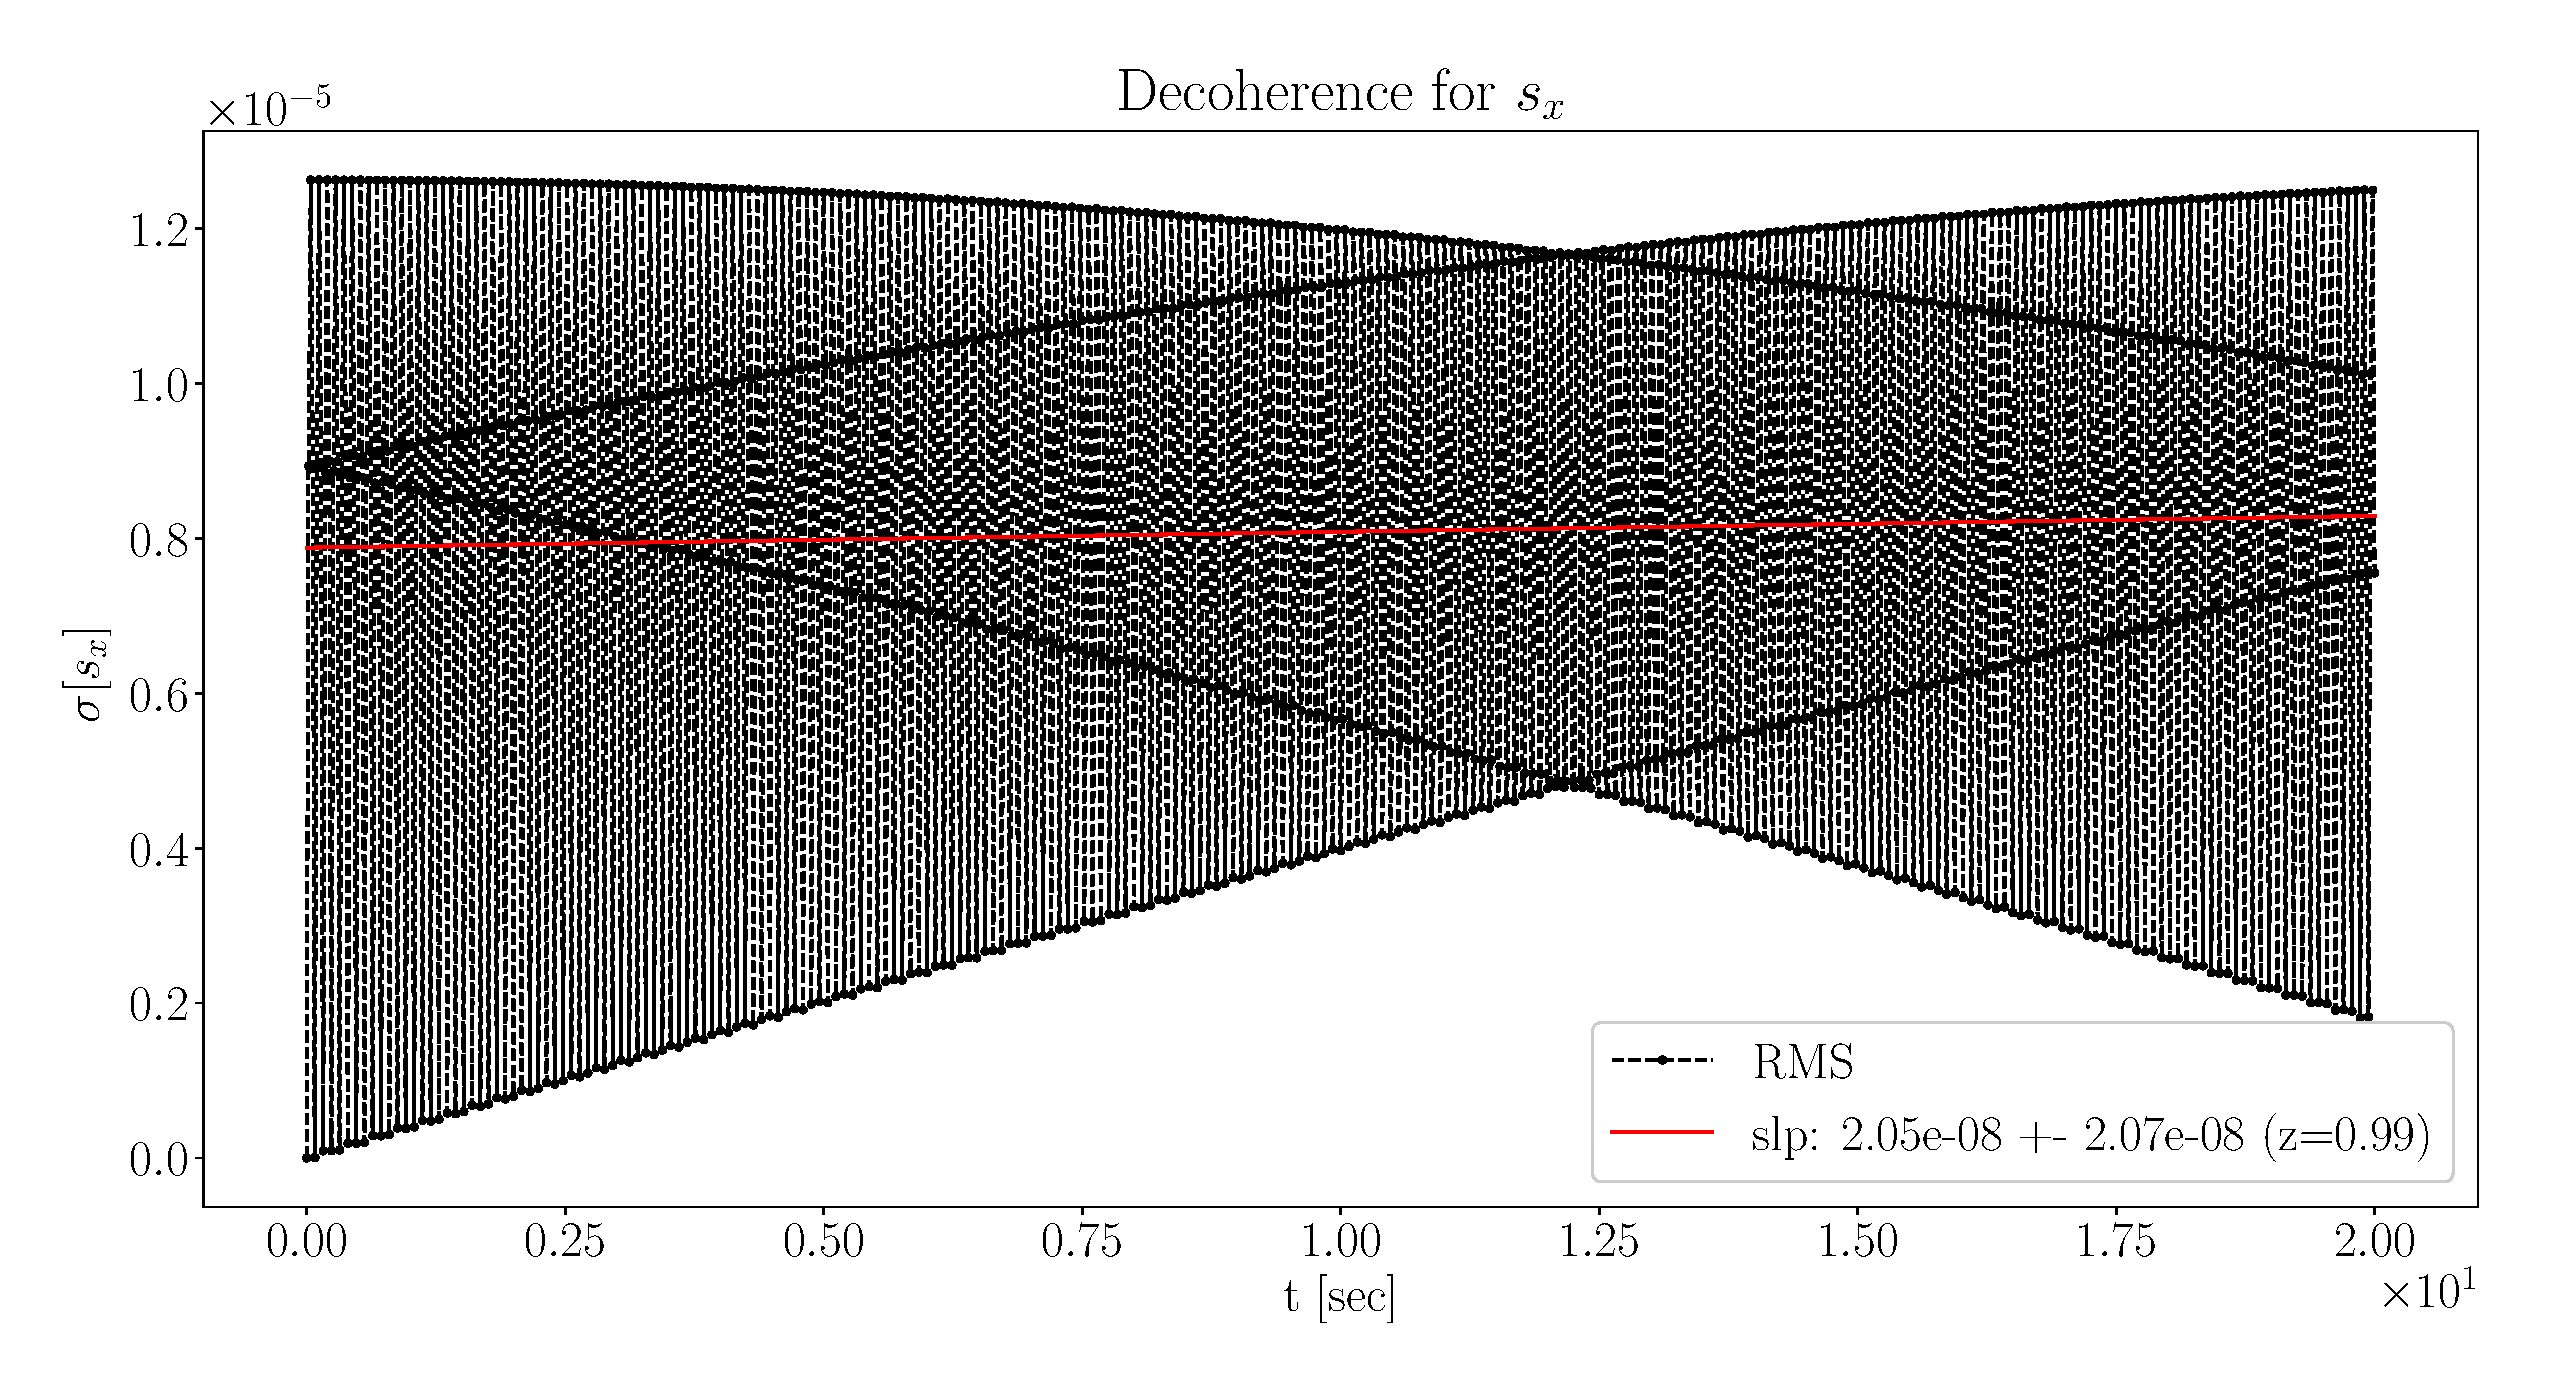
\includegraphics[height=.35\paperheight]{images/decoh_sim/SX_decoh_20sec_unopt}
		\caption{Sextupoles off}
	\end{subfigure}
	\begin{subfigure}{\linewidth}
		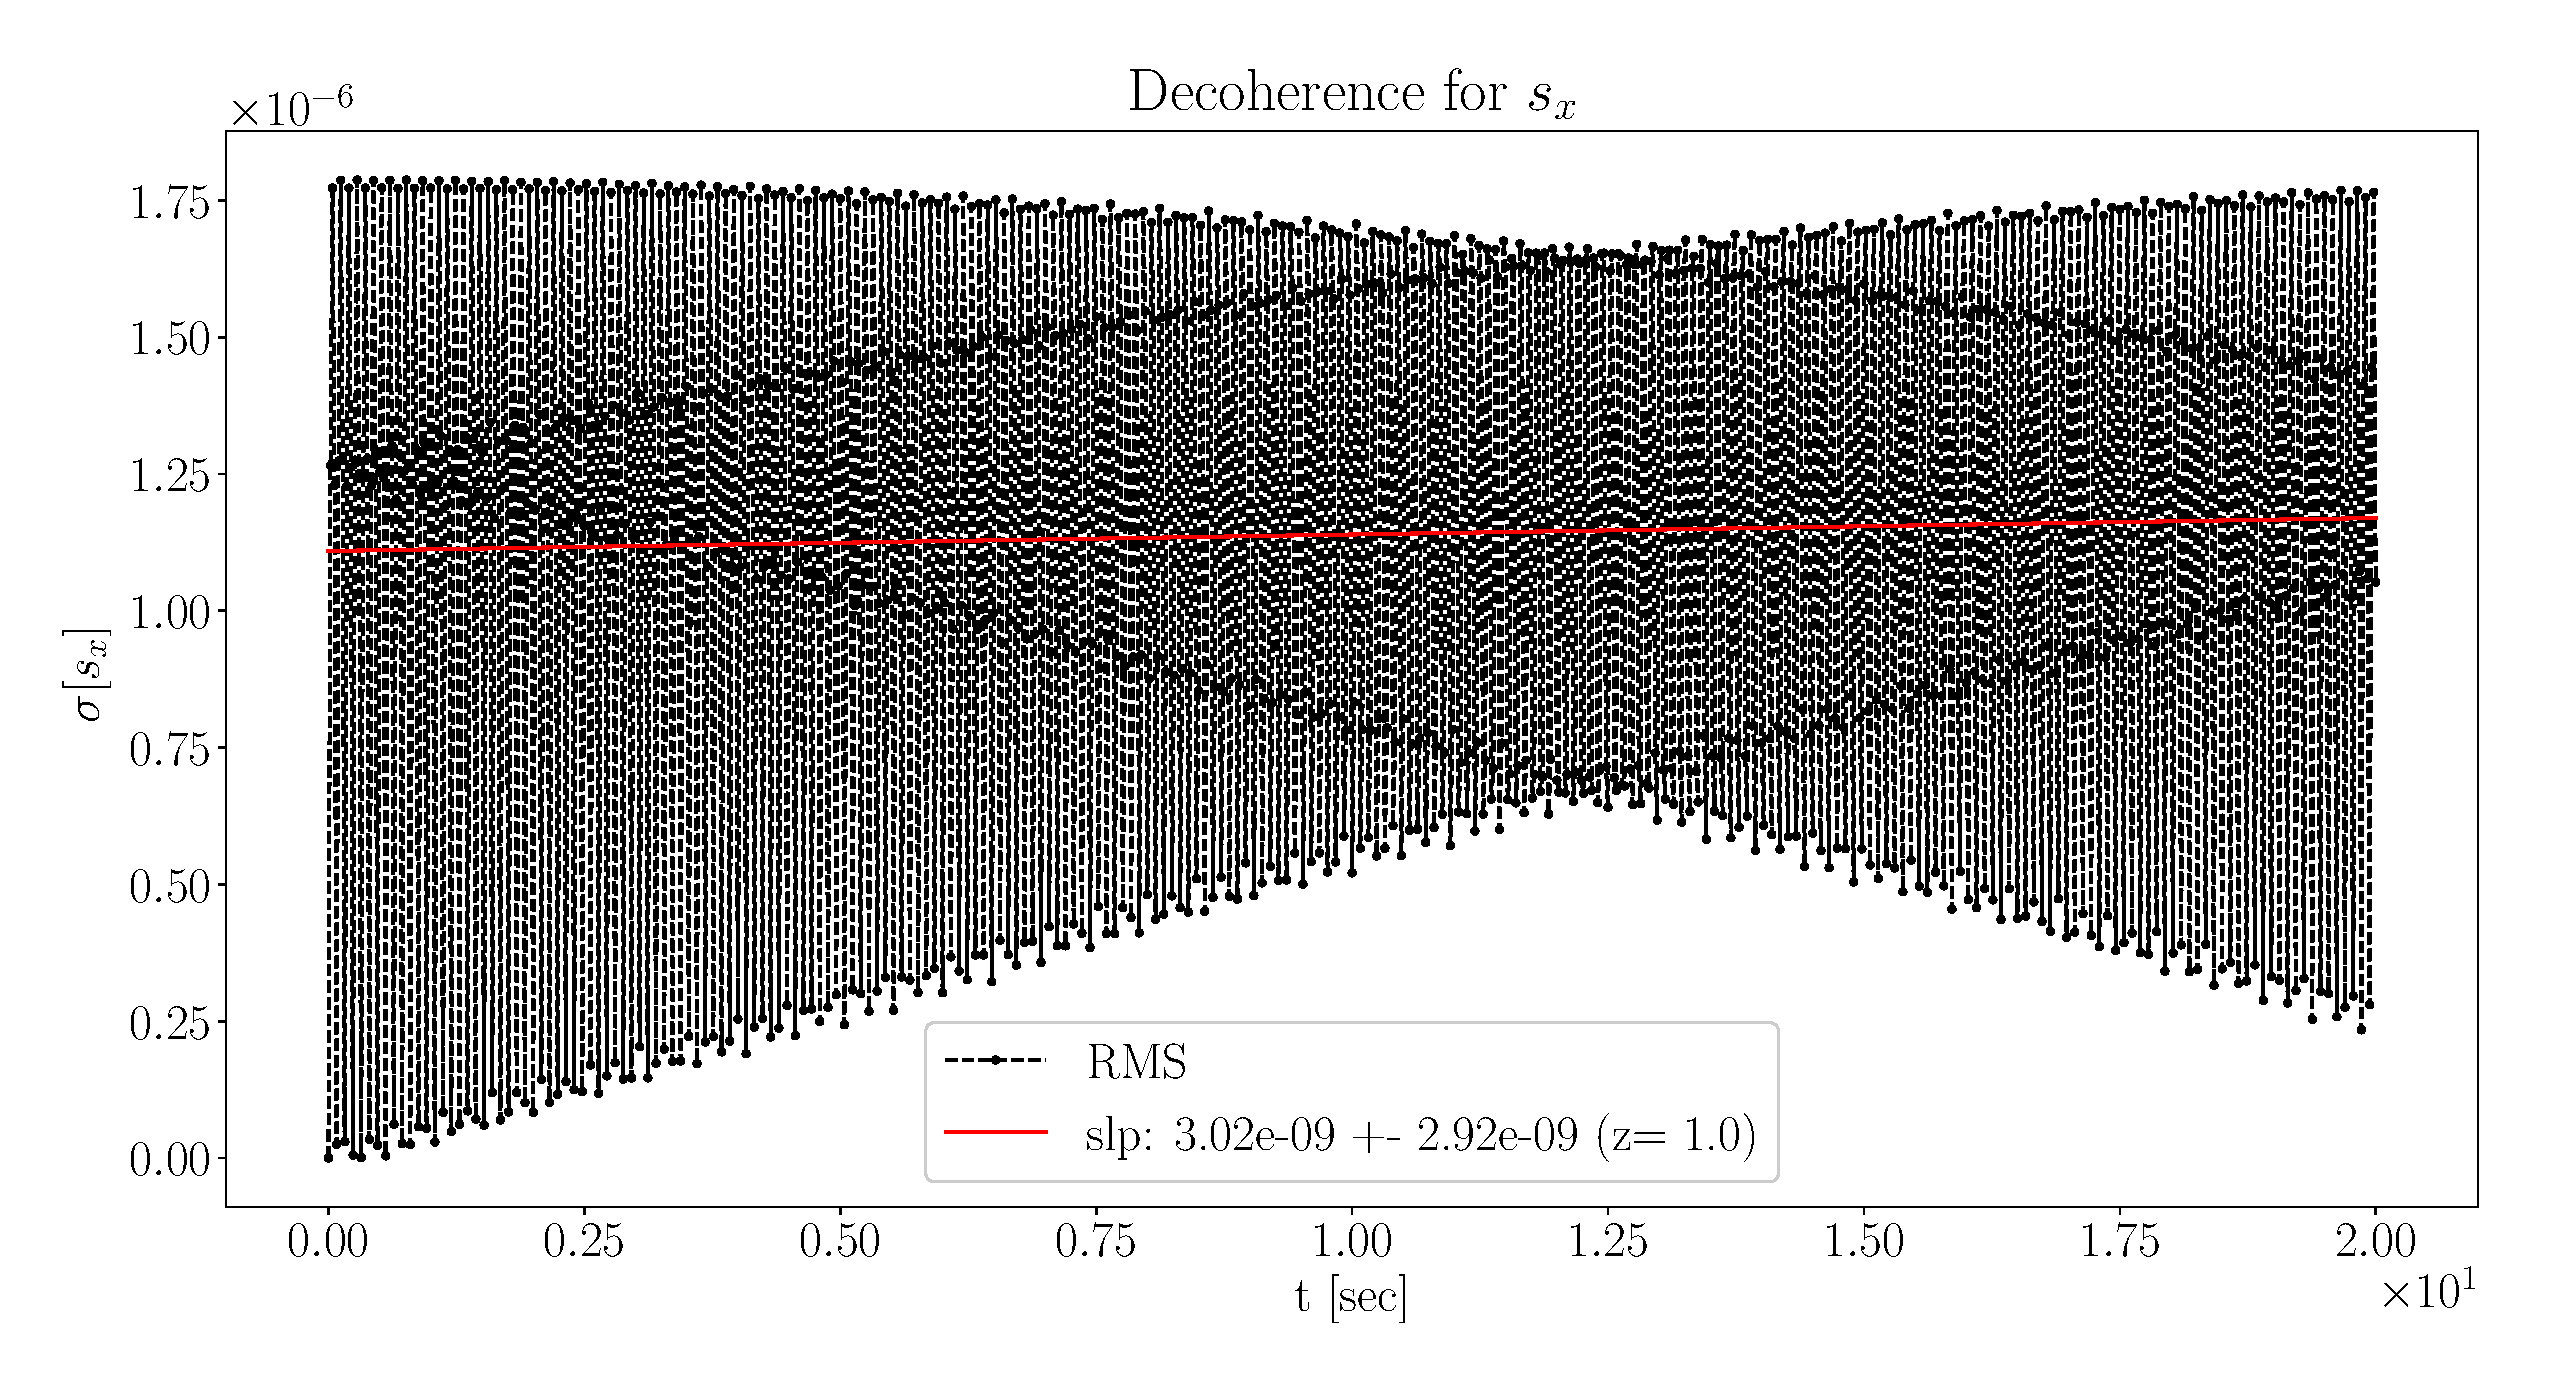
\includegraphics[height=.35\paperheight]{images/decoh_sim/SX_decoh_20sec_opt}
		\caption{Sextupoles on}
	\end{subfigure}
	\caption{Standard deviation of the radial spin vector component distribution in a bunch.\label{fig:decoh:SX_SD}}
\end{figure}

\begin{figure}[h!]
	\centering
	\begin{subfigure}{\linewidth}
		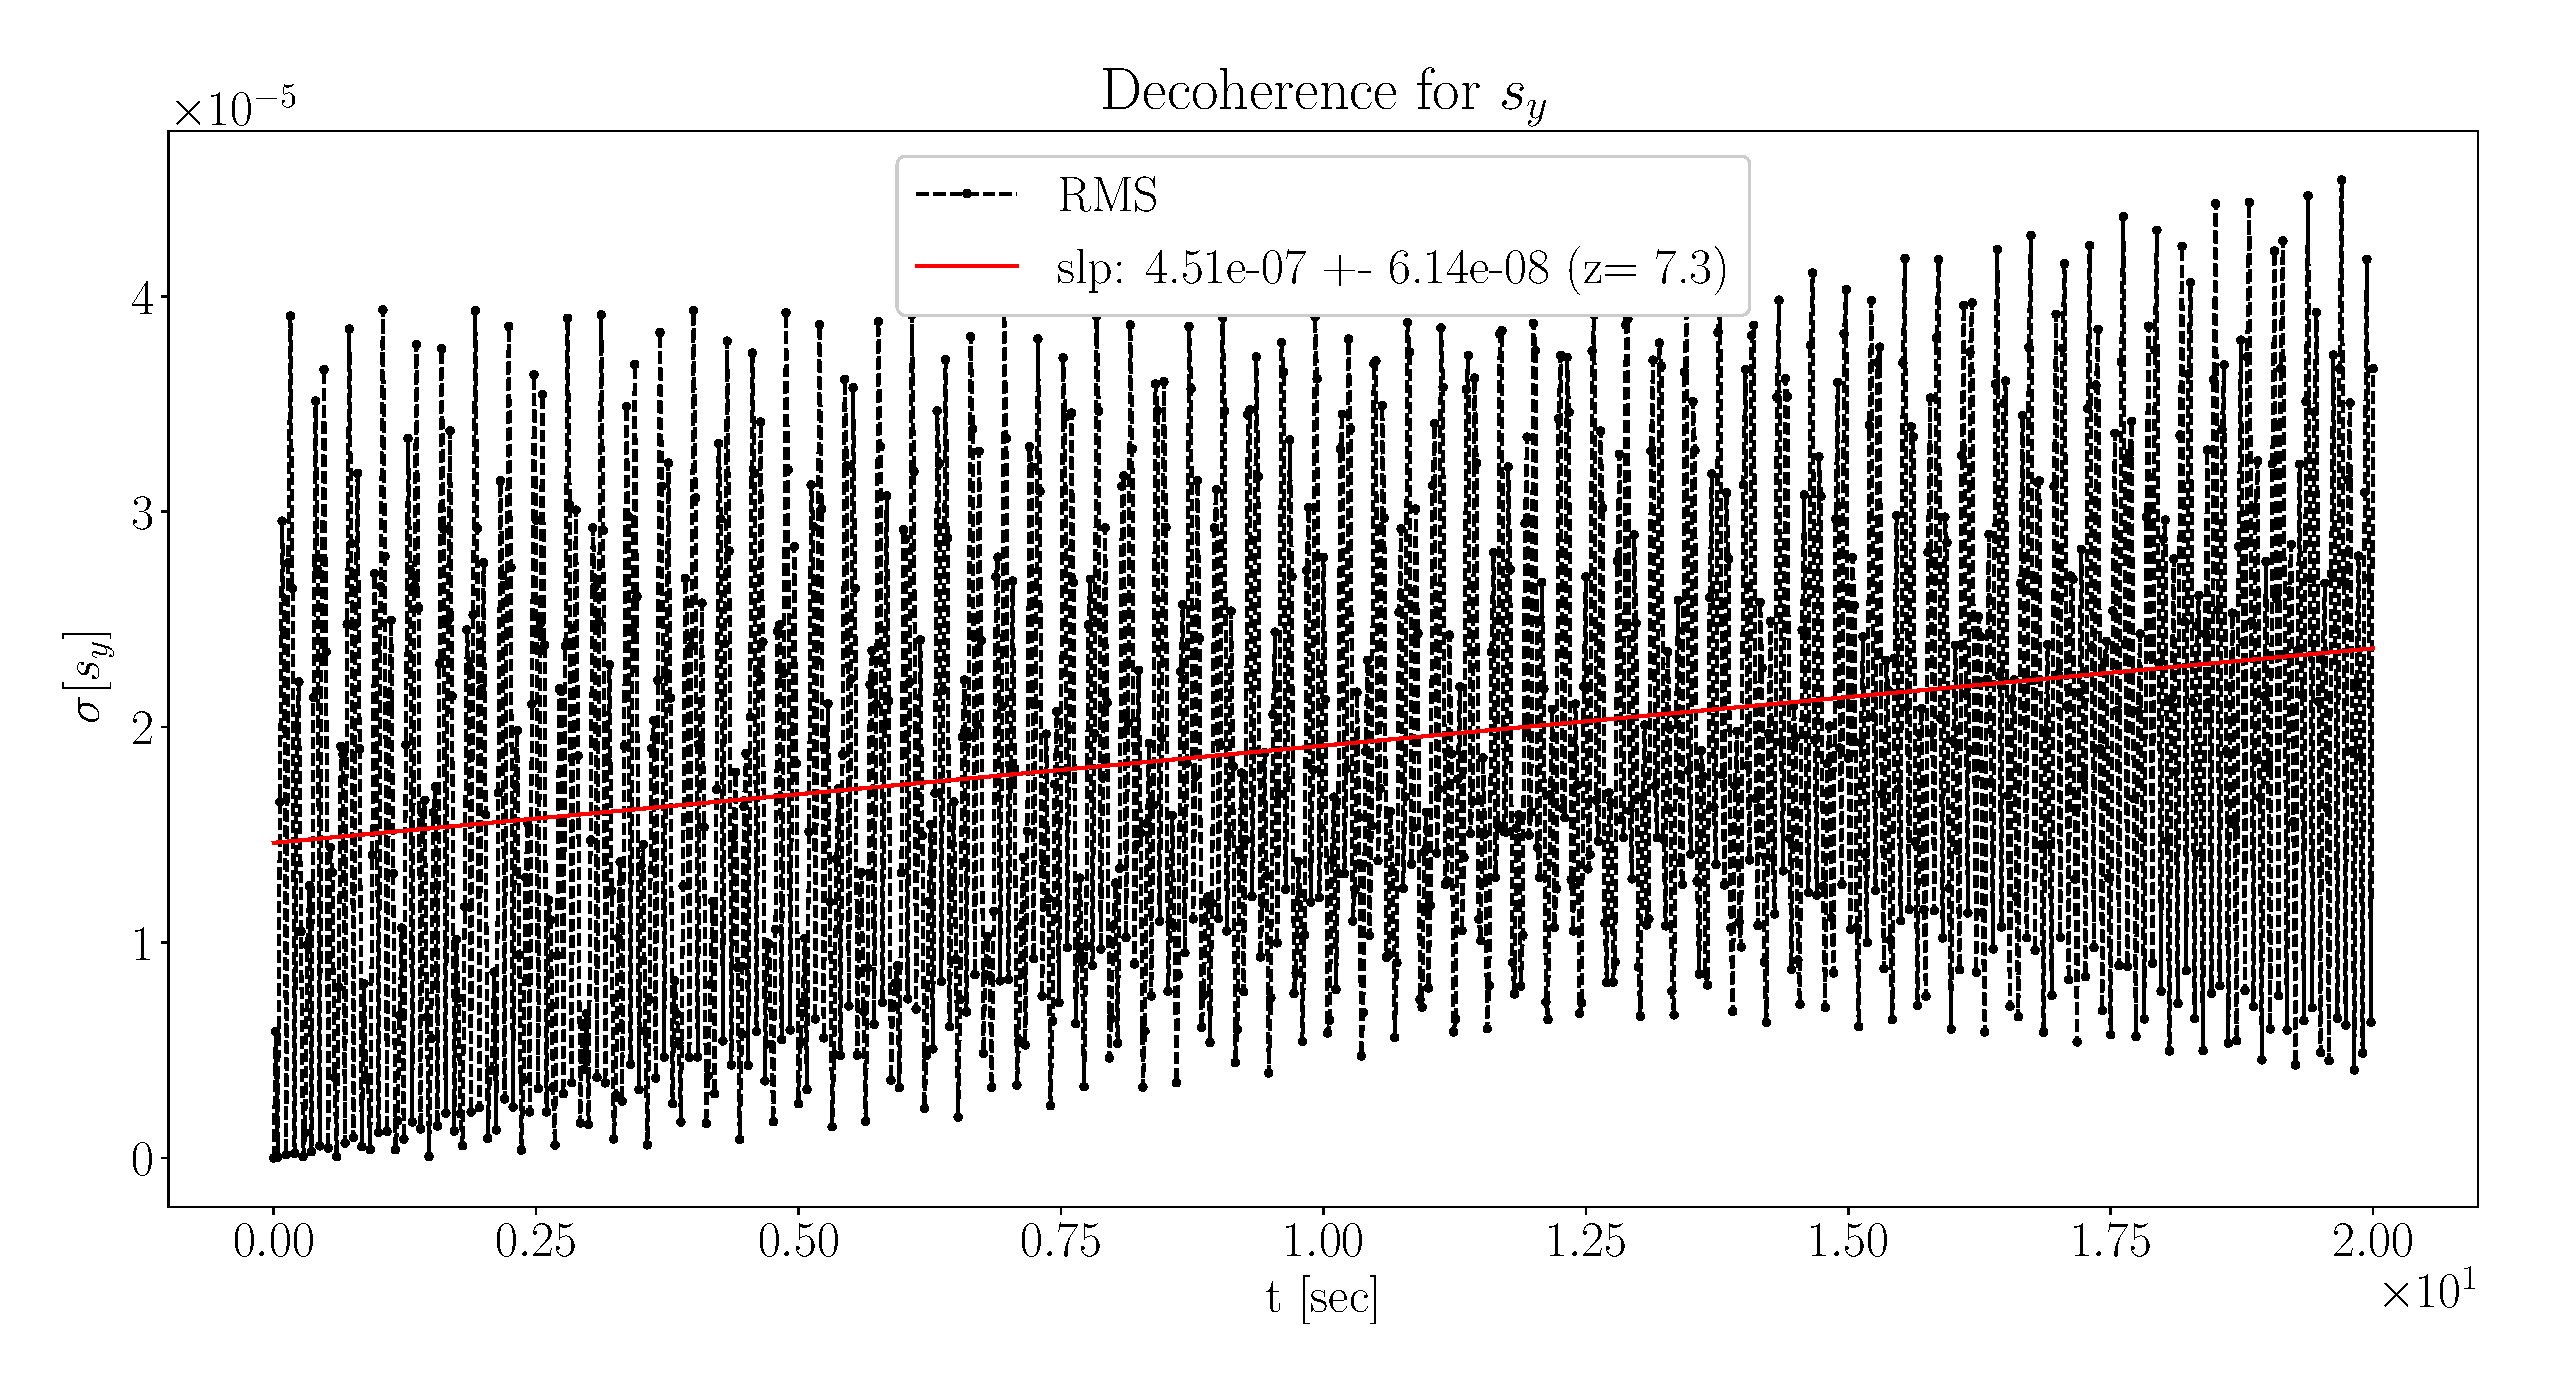
\includegraphics[height=.35\paperheight]{images/decoh_sim/SY_decoh_20sec_unopt}
		\caption{Sextupoles off}
	\end{subfigure}
	\begin{subfigure}{\linewidth}
		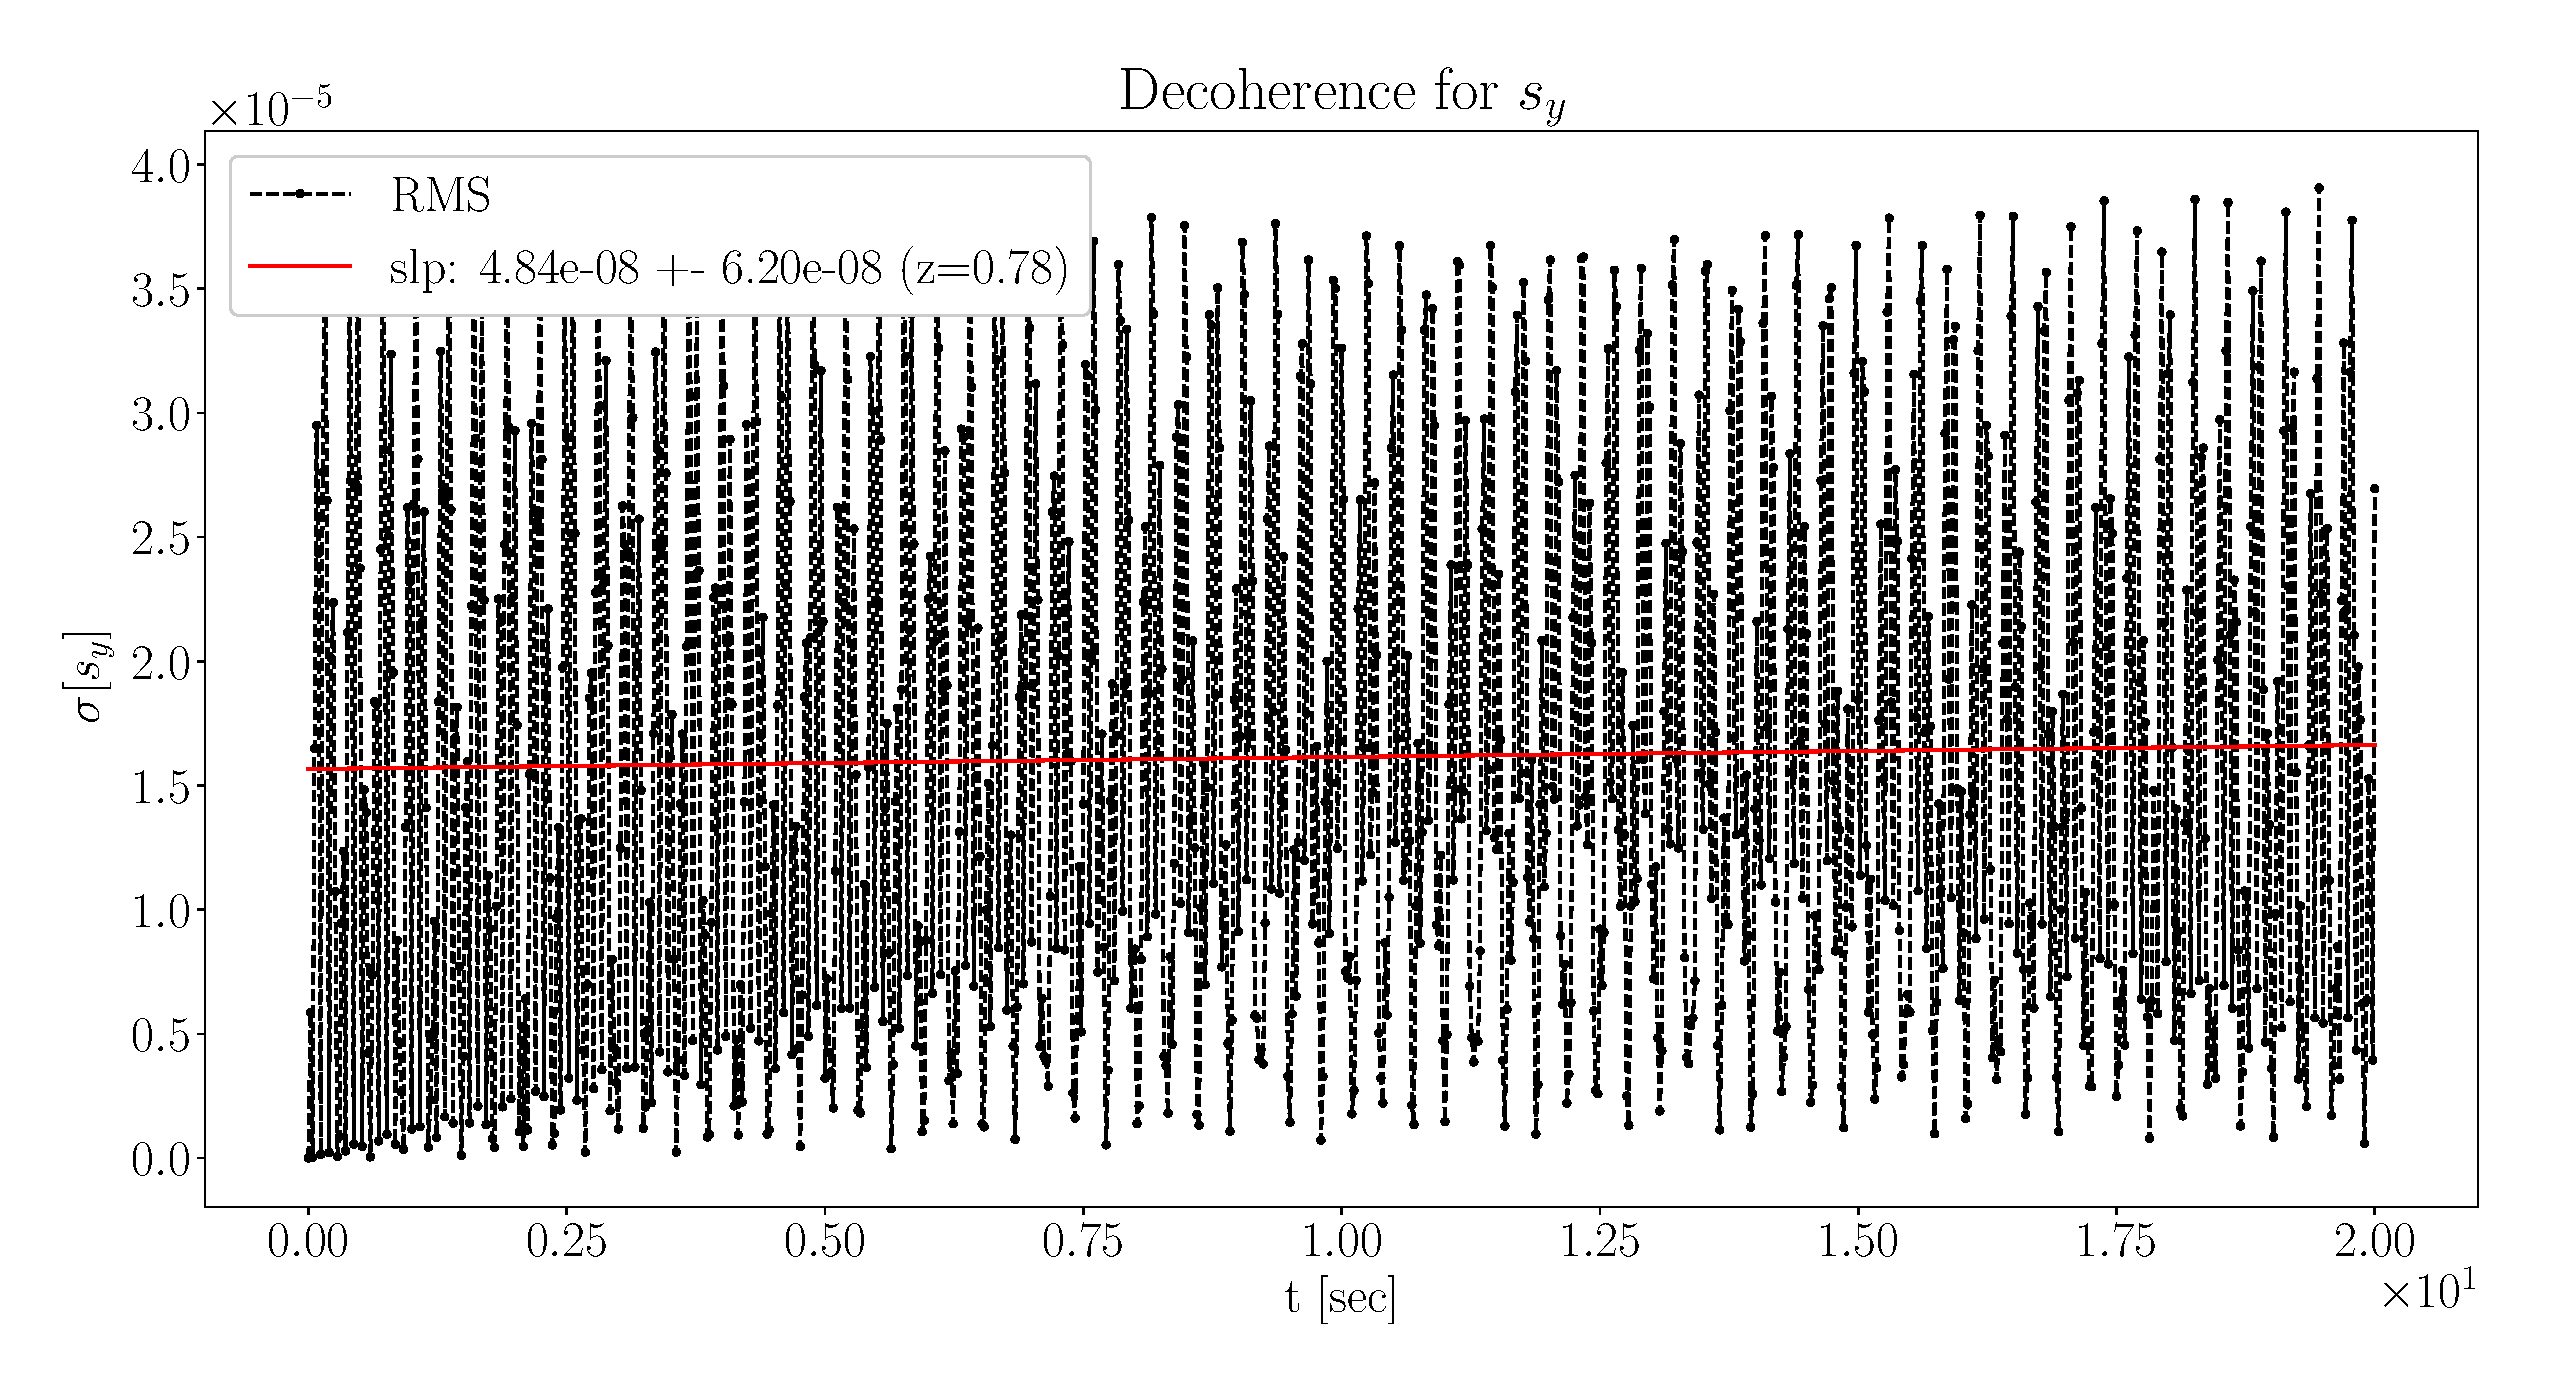
\includegraphics[height=.35\paperheight]{images/decoh_sim/SY_decoh_20sec_opt}
		\caption{Sextupoles on}
	\end{subfigure}
	\caption{Standard deviation of the radial spin vector component distribution in a bunch.\label{fig:decoh:SY_SD}}
\end{figure}

\subsection{Analysis of spin decoherence in an imperfect lattice}\label{sec:decoh:sim-imperfect}
The following tests were done with a planar bunch of 30 particles injected into a FS lattice
with E+B elements tilted about the optic axis by angles picked from $N(0, 5\cdot10^{-4})$ radians.

The beam particles were normally-distributed in the vertical plane $y-z$ along the $\hat y$-axis
as $y\sim N(y_0, 0.1)$ mm (all other phase space coordinates are zero). The offset $y_0$ varied in the
range $[-1, +1]$ mm. Initially all particles' spins were longitudinally oriented $\vec S(t=0) = (0,0,1)$.

We also varied the value $G_Y$ of the GSY sextupole.
$G_Y$ varied in the range $[G_Y^0 - 5\cdot10^{-3}, G_Y^0 + 5\cdot10^{-3}]$, where
$G_Y^0=-5.77\cdot 10^{-4}$ is the optimal gradient for this particular imperfection distribution.
The value $G_Y^0$ was found by minimizing the coefficient $a_2$
of the Taylor expansion $\nu_s(y) \approx a_0 + a_1\cdot y + a_2\cdot y^2 + O(y^3)$.

There were 10 injections at each value of $G_Y$.

To ensure the stability of the TSS procedure of COSY Infinity~\cite{COSYINF:Manual:BeamPhys},
the beam was injected at 270 MeV (the strict FS occurs at 270.0092 MeV), and the orbital and
spin transfer matrices were built up to the third order Taylor expansion. 

After that the beam is tracked through the lattice for $1.2\cdot10^6$ turns, which is approximately
equivalent to 1.2 seconds. Data used in the analysis were collected every 800 turns.

What we collected:
\begin{enumerate*}[\itshape a\upshape)]
	\item TSS procedure results: spin tune ($\nu_s$)  and the ISA ($\bar n$) components, и
	\item spin $(S_X, S_Y, S_Z)$ and phase space $(X,A,Y,B,T,D)$ vector components.
\end{enumerate*}
We also recorded the Taylor expansions of $\nu_s$, $\nbar$, orbital, and spin transfer matrices
of the lattice at each $G_Y$ value.

From the spin vector component data we computed the ensemble polarization:
\begin{equation}\label{eq:polarization_formula}
\vec P = \frac{\sum_i\vec s_i}{|\sum_i\vec s_i|}.
\end{equation}

Its vertical component is fitted by $f(t; a,f,\phi) = a\cdot \sin(2\pi\cdot
f\cdot t + \phi)$, where all three parameters $(\hat a, \hat f, \hat\phi)$ are estimated.  

\subsubsection{Sextupole field effect on spin tune and invariant spin axis}
In Figure~\ref{decoh:fig:ST_vs_y0_GSY} we showed the dependence of spin tune on the particle's
vertical offset from the reference orbit: $\nu_s(y) \approx a_0 + a_1\cdot y + a_2\cdot y^2 + O(y^3)$.
In Figure~\ref{decoh:fig:full:ST_vs_y0_GSY} one can observe the unbending of the parabola when
$G_Y \rightarrow G_Y^0$.
\begin{figure}[h!]
	\centering
	\begin{subfigure}{\linewidth}
		\includegraphics[width=\linewidth]{images/decoh_sim/spin_tune_vs_offset}
		\caption{Full range.\label{decoh:fig:full:ST_vs_y0_GSY}}
	\end{subfigure}
	\begin{subfigure}{\linewidth}
		\includegraphics[width=\linewidth]{images/decoh_sim/spin_tune_vs_offset_zoom}
		\caption{Detalization.\label{decoh:fig:zoom:ST_vs_y0_GSY}}
	\end{subfigure}
	\caption{Spin tune $\nu_s$ as a function of the particle's vertical offset from the closed orbit.
          Color marks different $G_Y$ values.\label{decoh:fig:ST_vs_y0_GSY}}
\end{figure}

An equivalent dependence for the vetrical component of the ISA is shown
in Figure~\ref{decoh:fig:ny_vs_y0_GSY}. In Figure~\ref{decoh:fig:full:ny_vs_y0_GSY} we observe
that the ISA component behaves the same way as spin tune when $G_Y \rightarrow G_Y^0$.
Just as in the case of an ideal lattice, in Figure~\ref{decoh:fig:zoom:ny_vs_y0_GSY}
one can observe the presence of a linear term in $\nbar_y(y)$, insensitive to the sextupole fields.

\begin{figure}[h!]
	\centering
	\begin{subfigure}{\linewidth}
		\includegraphics[width=\linewidth]{images/decoh_sim/ny_vs_offset}
		\caption{Full range.\label{decoh:fig:full:ny_vs_y0_GSY}}
	\end{subfigure}
	\begin{subfigure}{\linewidth}
		\includegraphics[width=\linewidth]{images/decoh_sim/ny_vs_offset_zoom}
		\caption{Detalization.\label{decoh:fig:zoom:ny_vs_y0_GSY}}
	\end{subfigure}
	\caption{Vertical component $\bar n_y$ of the invariant spin axis as a function of the particle's
          vertical offset from the closed orbit.
          Color marks different $G_Y$ values\label{decoh:fig:ny_vs_y0_GSY}}
\end{figure}

In the figures above, the values of spin tune and ISA were computed as univariate functions
of the vertical offset; all other phase space coordinates were set to reference values. While analyzing
the tracker data we noted that the ISA components (as well as spin tune) of a particle do not oscillate,
as one would expect from the figures, but remain nearly constant. We hypothesized that the $\nu_s$ and $\nbar$
dependencies on the vertical offset and ite derivative ($y'\equiv a$) compensate each other when the particle
moves along a real trajeoctory. On the next figures we depicted $\nu_s$, $\nbar$ at their true phase space
trajectories in the storage ring.

In Figure~\ref{decoh:fig:yb_traj} are depicted the particle trajectories in the $(Y,B)$ phase plane,
obtained in tracking the particles through the imperfect lattice.
\begin{figure}[h!]
	\centering
	\includegraphics[width=\linewidth]{images/decoh_sim/YB-PHASE_SPACE_IMPERFECT_UNOPT}
	\caption{Particle trajectories in the $(Y,B)$ phase space.\label{decoh:fig:yb_traj}} 
\end{figure}

In Figures~\ref{decoh:fig:ST_on_traj}, \ref{decoh:fig:NX_on_traj}, \ref{decoh:fig:NY_on_traj}, and
\ref{decoh:fig:NZ_on_traj} are plotted, respectively: spin tune, the radial, vertical, and longitudinal
components of the ISA, computed at the trajectories plotted in Figure~\ref{decoh:fig:yb_traj}, in two cases:
\begin{enumerate*}[\itshape i\upshape)]
	\item sextupoles are turned off, and 
	\item GSY sextupoles are turned on.
\end{enumerate*}  

\begin{figure}[!h]
	\centering
	\begin{subfigure}{\linewidth}
		\includegraphics[width=\linewidth]{images/decoh_sim/ST_VS_YB_IMPERFECT_UNOPT}
		\caption{Sextupoles off.}
	\end{subfigure}
	\begin{subfigure}{\linewidth}
		\includegraphics[width=\linewidth]{images/decoh_sim/ST_VS_YB_IMPERFECT_OPTIM}
		\caption{Sextupoles on.}
	\end{subfigure}
	\caption{Particle spin tunes computed at their trajectories
          in an imperfect FS lattice.\label{decoh:fig:ST_on_traj}}
\end{figure}

\begin{figure}[!h]
	\centering
	\begin{subfigure}{\linewidth}
		\includegraphics[width=\linewidth]{images/decoh_sim/NX_VS_YB_IMPERFECT_UNOPT}
		\caption{Sextupoles off.}
	\end{subfigure}
	\begin{subfigure}{\linewidth}
		\includegraphics[width=\linewidth]{images/decoh_sim/NX_VS_YB_IMPERFECT_OPTIM}
		\caption{Sextupoles on.}
	\end{subfigure}
	\caption{Particle's radial ISA components computed at their trajectories
          in an imperfect FS lattice.\label{decoh:fig:NX_on_traj}}
\end{figure}

\begin{figure}[!h]
	\centering
	\begin{subfigure}{\linewidth}
		\includegraphics[width=\linewidth]{images/decoh_sim/NY_VS_YB_IMPERFECT_UNOPT}
		\caption{Sextupoles off.}
	\end{subfigure}
	\begin{subfigure}{\linewidth}
		\includegraphics[width=\linewidth]{images/decoh_sim/NY_VS_YB_IMPERFECT_OPTIM}
		\caption{Sextupoles on.}
	\end{subfigure}
	\caption{Particle's vertical ISA components computed at their trajectories
          in an imperfect FS lattice.\label{decoh:fig:NY_on_traj}}
\end{figure}

\begin{figure}[!h]
	\centering
	\begin{subfigure}{\linewidth}
		\includegraphics[width=\linewidth]{images/decoh_sim/NZ_VS_YB_IMPERFECT_UNOPT}
		\caption{Sextupoles off.}
	\end{subfigure}
	\begin{subfigure}{\linewidth}
		\includegraphics[width=\linewidth]{images/decoh_sim/NZ_VS_YB_IMPERFECT_OPTIM}
		\caption{Sextupoles on.}
	\end{subfigure}
	\caption{Particle's longitudinal ISA components computed at their trajectories
          in an imperfect FS lattice.\label{decoh:fig:NZ_on_traj}}
\end{figure}

From the analysis of the figures, we can gather the following:
\begin{enumerate}
\item in the sextupoles-off case, both $\nu_s$ and the direction of $\nbar$ are mostly (to the
  linear Taylor expansion term) fixed by the value of the particle's transverse emittance;
\item in the sextupoles-on case, the mean levels of $\nu_s$ and $\nbar$ of different particles come
  together, and the betatron motion effect, related to the presence of a linear Taylor expansion term,
  becomes apparent.
\end{enumerate}
Hence, Figures~\ref{decoh:fig:NX_on_traj} and~\ref{decoh:fig:NY_on_traj} are evidence that not only are the
\textbf{frequencies} but also the \textbf{directions} of the beam particles' spin precession angular
velocity vectors are equalized when sextupole fields are used to suppress spin decoherence. The
longitudinal component of the ISA is insensitive to the sextupole fields, as evicdenced
by Figure~\ref{decoh:fig:NZ_on_traj}.

In Figure~\ref{decoh:fig:nbar_vs_ST} are shown the dependencies of the radial and vertical ISA components'
mean levels on the particle's mean spin tune level. Based on this figure, we conclude
in section~\ref{sec:spin_stune_traj_equ:B_form} that particles having equal effective Lorentz factor values
are equivalent in terms of their spin dynamics in the general (direction and magnitude of the spin precession
angular velocity vector) sense.~\footnote{At least this seems to be true when operating
  in the frozen spin regime.}
\begin{figure}[!h]
	\centering
	\includegraphics[width=\linewidth]{images/decoh_sim/mean_n_bar_vs_spin_tune}
	\caption{Mean level of the radial and vertical ISA components versus the correcponding
          value of spin tune.\label{decoh:fig:nbar_vs_ST}}
\end{figure}

\subsection{Analysis of the sextupole spin decoherence suppression mechanism}\label{sec:sext_decoh_suppression_effect_analysis}
From equations~\eqref{eq:spin_tune_vs_gamma} and~\eqref{eq:EquLevMom_shift}, the dependence of spin tune of the
particle equilibrium energy can be expressed as:
\[
\nu_s = G\gamma_0 + G\frac{\gamma_0^2-1}{\gamma_0}\cdot C_0\cdot f_1(\epsilon_x, \epsilon_y, Q_x, Q_y)+ G\frac{\gamma_0^2-1}{\gamma_0}\cdot C_0\cdot f_2(\alpha_1, \avg{\Delta K/K}^2),
\]
where $C_0$ is a constant, $f_1$ and $f_2$ are defined in equation~\eqref{eq:EquLevMom_shift}.

Since a betatron-oscillating particle does also synchrotron oscillations, the effct of sextupole fields on it
is a superposition of effects. A particle injected onto the reference orbit, but having an initial energy
offset, does only synchrotron oscillations. Consequently, sextupole fields affect its spin tune by only
modifying the momentum compaction factor, i.e. $f_2$.

In view of that, we carried out a simulation in which we consecutively injected two beams of 30 particles:
in the first one, the D-bunch, particles were distributed as $\delta\sim N(0, 0.5\cdot 10^{-6})$, 
in the second one, the Y-bunch, as $y\sim N(0, 0.5)$ mm. All the other phase space coordinates were initially
set to zero.

The bunches were injected into the ideal FS lattice in order to exclude effects associated with perturbations
of non-reference orbits. For the D-bunch, only the GSD sextupoles were turned on; for the Y-bunch -- GSY. The
sextupole gradients were varied $\pm 5\cdot 10^{-3}$ of the corresponding family's optimal gradient value.

Spin tracking was done for $1.2\cdot 10^6$ turns, data were recorded every 800 turns.

In Figure~\ref{fig:long_PS_sext_settings} are plotted the particles' longitudinal phase space portraits. 
We see that the D-bunch phase portraits are practically all centered at the same point,~\footnote{When zooming 	in, one can see that the ellipse centers are slightly different, but this difference is insensitive to
	the sextupole gradient value, and most likely is the result of finite statistics.} and that their 
emittances do not change when the sextupole strength is varied.

At the same time, the Y-bunch phase portraits vary with the sextupole field strength. We observe that the 
the ellipse centers (i.e. the equilibrium energy levels) are the most compressed at a gradient value that is
\textbf{not} optimal (the phase portraits for the latter are drawn in the middle panel). This observation
was what motivated us to try to inject the D-bunch in the first place. We explain this observation by the
superposition of the orbit length and momentum compaction factor effects.

\begin{figure}[h]
	\centering
	\begin{subfigure}{\linewidth}
		\includegraphics[width=\linewidth]{images/decoh_sim/propdef/long_phase_space_for_sext_settings_D}
		\caption{D-bunch phase portraits.}
	\end{subfigure}
	\begin{subfigure}{\linewidth}
		\includegraphics[width=\linewidth]{images/decoh_sim/propdef/long_phase_space_for_sext_settings_Y}
		\caption{Y-bunch phase portraits.}
	\end{subfigure}
	\caption{Longitudinal phase space particle portraits. Asterisks mark the ellipse centers.
		Colors mark trajectories of particles with differing initial vertical offset from the reference orbit.\label{fig:long_PS_sext_settings}}
\end{figure}

For a more thorough analysis of the sextupoel field effects on the functions $f_1$ and $f_2$ we plotted the
dependencies of the particles' mean spin tune levels on their equilibrium energy levels at different
sextupole field strengths (Figure~\ref{fig:ST_vs_dkok_for_sext_strenghts}). One can see from the figure 
that the point distribution density in the D-bunch plot does not vary with the gradient value; the only thing 
that changes is the functional dependence of spin tune on the equilibrium energy level, as is expected from
the functional form of $f_2$ (cf. section~\ref{chpt1:FS-methods:effective-Lorentz-factor}). Hence, the 
signature of the sextupole field's momentum compaction effect is the change in the functional form of
 $\avg{\nu_s} = f(\avg{\Delta K/K})$.

In the Y-bunch plot one observes two effects: both the point distribution density (i.e. the beam's longitudinal emittance) and the functional form of $\avg{\nu_s}(\avg{\Delta K/K})$ change.

\begin{figure}[h]
	\centering
	\begin{subfigure}{\linewidth}
		\includegraphics[width=\linewidth]{images/decoh_sim/propdef/stune_vs_dkok_SS_D}
		\caption{For the D-bunch.}
	\end{subfigure}
	\begin{subfigure}{\linewidth}
		\includegraphics[width=\linewidth]{images/decoh_sim/propdef/stune_vs_dkok_SS_Y}
		\caption{For the Y-bunch.}
	\end{subfigure}
	\caption{Particle mean spin tune level as a function of its equilibrium level energy at different sextupole strengths.\label{fig:ST_vs_dkok_for_sext_strenghts}}
\end{figure}

\paragraph{Conclusion:} The simulation confirms statements~\eqref{eq:Sext_compaction_effect} and~\eqref{eq:Sext_OL_effect}.


\section{Ошибки неидеальности ускорителя}\label{chpt3:imperfections}
Systematic errors due to physical imperfections of the accelerator lattice, including
optical element misalignments, are causative to an EDM-faking signal 
related to MDM spin precession~\cite[з.~230]{Eremey:Thesis} Rotational magnet misalignments 
aer particularly problematic in this respect, since they induce parasitic horizontal magnetic field
components $B_x$ and $B_z$, both of which precess spin in the vertical plane; the one in which
the EDM is searched for.

Y. Senichev made analytical estimates~\cite{Senichev:FDM}  of the radial component of
the spin precession angular velocity vector. From the T-BMT equation, and the expression for
the Lorentz force, the radial component can be expressed as 
\begin{equation}
\SD{\W_x^{MDM}} = \frac{q}{m\gamma}\frac{G+1}{\gamma}\frac{\SD{B_x}}{\sqrt{n}},
\end{equation}
where $n$ is the number of tilted spin-rotator elements,~\footnote{The estimates were made for
the FS lattice described in section~\ref{chpt2:lattice:FS_BNL}} and $\SD{B_x} = B_y \SD{\delta h}/L$, 
with the misalignment error standard deviation $\SD{\delta h}$. Assuing $\SD{\delta h} = 100$ $\mu$m, 
and the spin-rotator length $L=1$ m, $\SD{\W_x^{MDM}} \approx 100$ rad/sec.~\cite{Senichev:FDM}

We analyzed the particle spin dynamics in the imperfect FS and QFS lattices using the COSY Infinity code. 
Our simulation results tend to confirm the above estimates.


\paragraph{Imperfection field implementation}\label{chpt3:imperfections:implementation}
When implementing machine imperfections we followed recommendations given in~\cite[p.~235]{Eremey:Thesis}. 
A small perturbation of the magnetic field acts like a proportional rotation of the spin vector.
For this reason we implemented the E+B element tilt as a product between the element's spin transfer matrix
and the corresponding rotation matrix, a ``spin kick.'' Such an implementation guarantees the preservation of 
the closed orbit. This orbit preservation is physically grounded in the fact that when a spin-rotator
is tilted, there emerges a compensating electric field keeping the Lorentz force constant.

According to equation~\eqref{eq:TBMT_MDM}, a change in the MDM precession angular velocity
associated with the presence of a parasitic magnetic field $(B_x, 0, B_z)$ is
\begin{align*}
	\Delta\W_{MDM} &= \frac qm G \cdot (B_x, 0, B_z),
	\intertext{hence the spin kick angle}
	\Theta_{kick} &= t_0\Delta\W_{MDM},
\end{align*}
where $t_0 = L/v_0$ is the reference particle's time of flight through the element.

\subsection{Tilt distribution dependence} \label{chpt3:imperfections:magnitude}
This series of simulations was carried out in order to prove (or reject) the validity of two theses
concerning the machine imperfection systematic error:
\begin{enumerate*}[(1)]
	\item the induced MDM spin precession angular velocity component is independent of the particular
	element tilt distribution, and depends only on the mean tilt angle; and
	\item this dependence is linear.
\end{enumerate*}

The simulation was set up as follows: in the FS lattice described in section~\ref{chpt2:lattice:FS_BNL} 
 E+B elements were randomly tilted about the optic axis by angles $\Theta_{tilt}$.
 After building the third-order spin and orbital transfer maps, we computed the Taylor expansions of the
 spin tune and spin precession axis (SPA). The zero-order terms of the Taylor expansions represent the spin tune and SPA
 of the reference particle.
 
 The reference particle spin precession angular velocity is calculated 
 according to equation:~\cite[p.~4]{COSY:SpinTuneMapping}
\[
\vec\W = 2\pi/\tau_0\cdot \nu_s \cdot \bar n,
\]
where $\tau_0 = f^{-1}_{rev} = 10^{-6}$ seconds is the particle's time of flight through the full lattice.

The simulation was carried out 11 times; each time the spin-rotator tilt angles were picked
from a normal distribution $N(\mu_0\cdot(i-5), \sigma_0)$, where 
$\mu_0 = 10\cdot \sigma_0 = 10^{-4}$ rad, $i\in\lbrace0,\dots, 10\rbrace$. The simulation
results are plotted in Figure~\ref{fig:Linearity_test_shifting_gauss}.

\begin{figure}[!h]
	\centering
	\begin{subfigure}{\linewidth}
		\includegraphics[height=.35\paperheight]{images/fake_signal_sim/linearity_test_shifting_gauss_nbar}
		\caption{Spin precession axis $\nbar$ components.}
	\end{subfigure}
	\begin{subfigure}{\linewidth}
		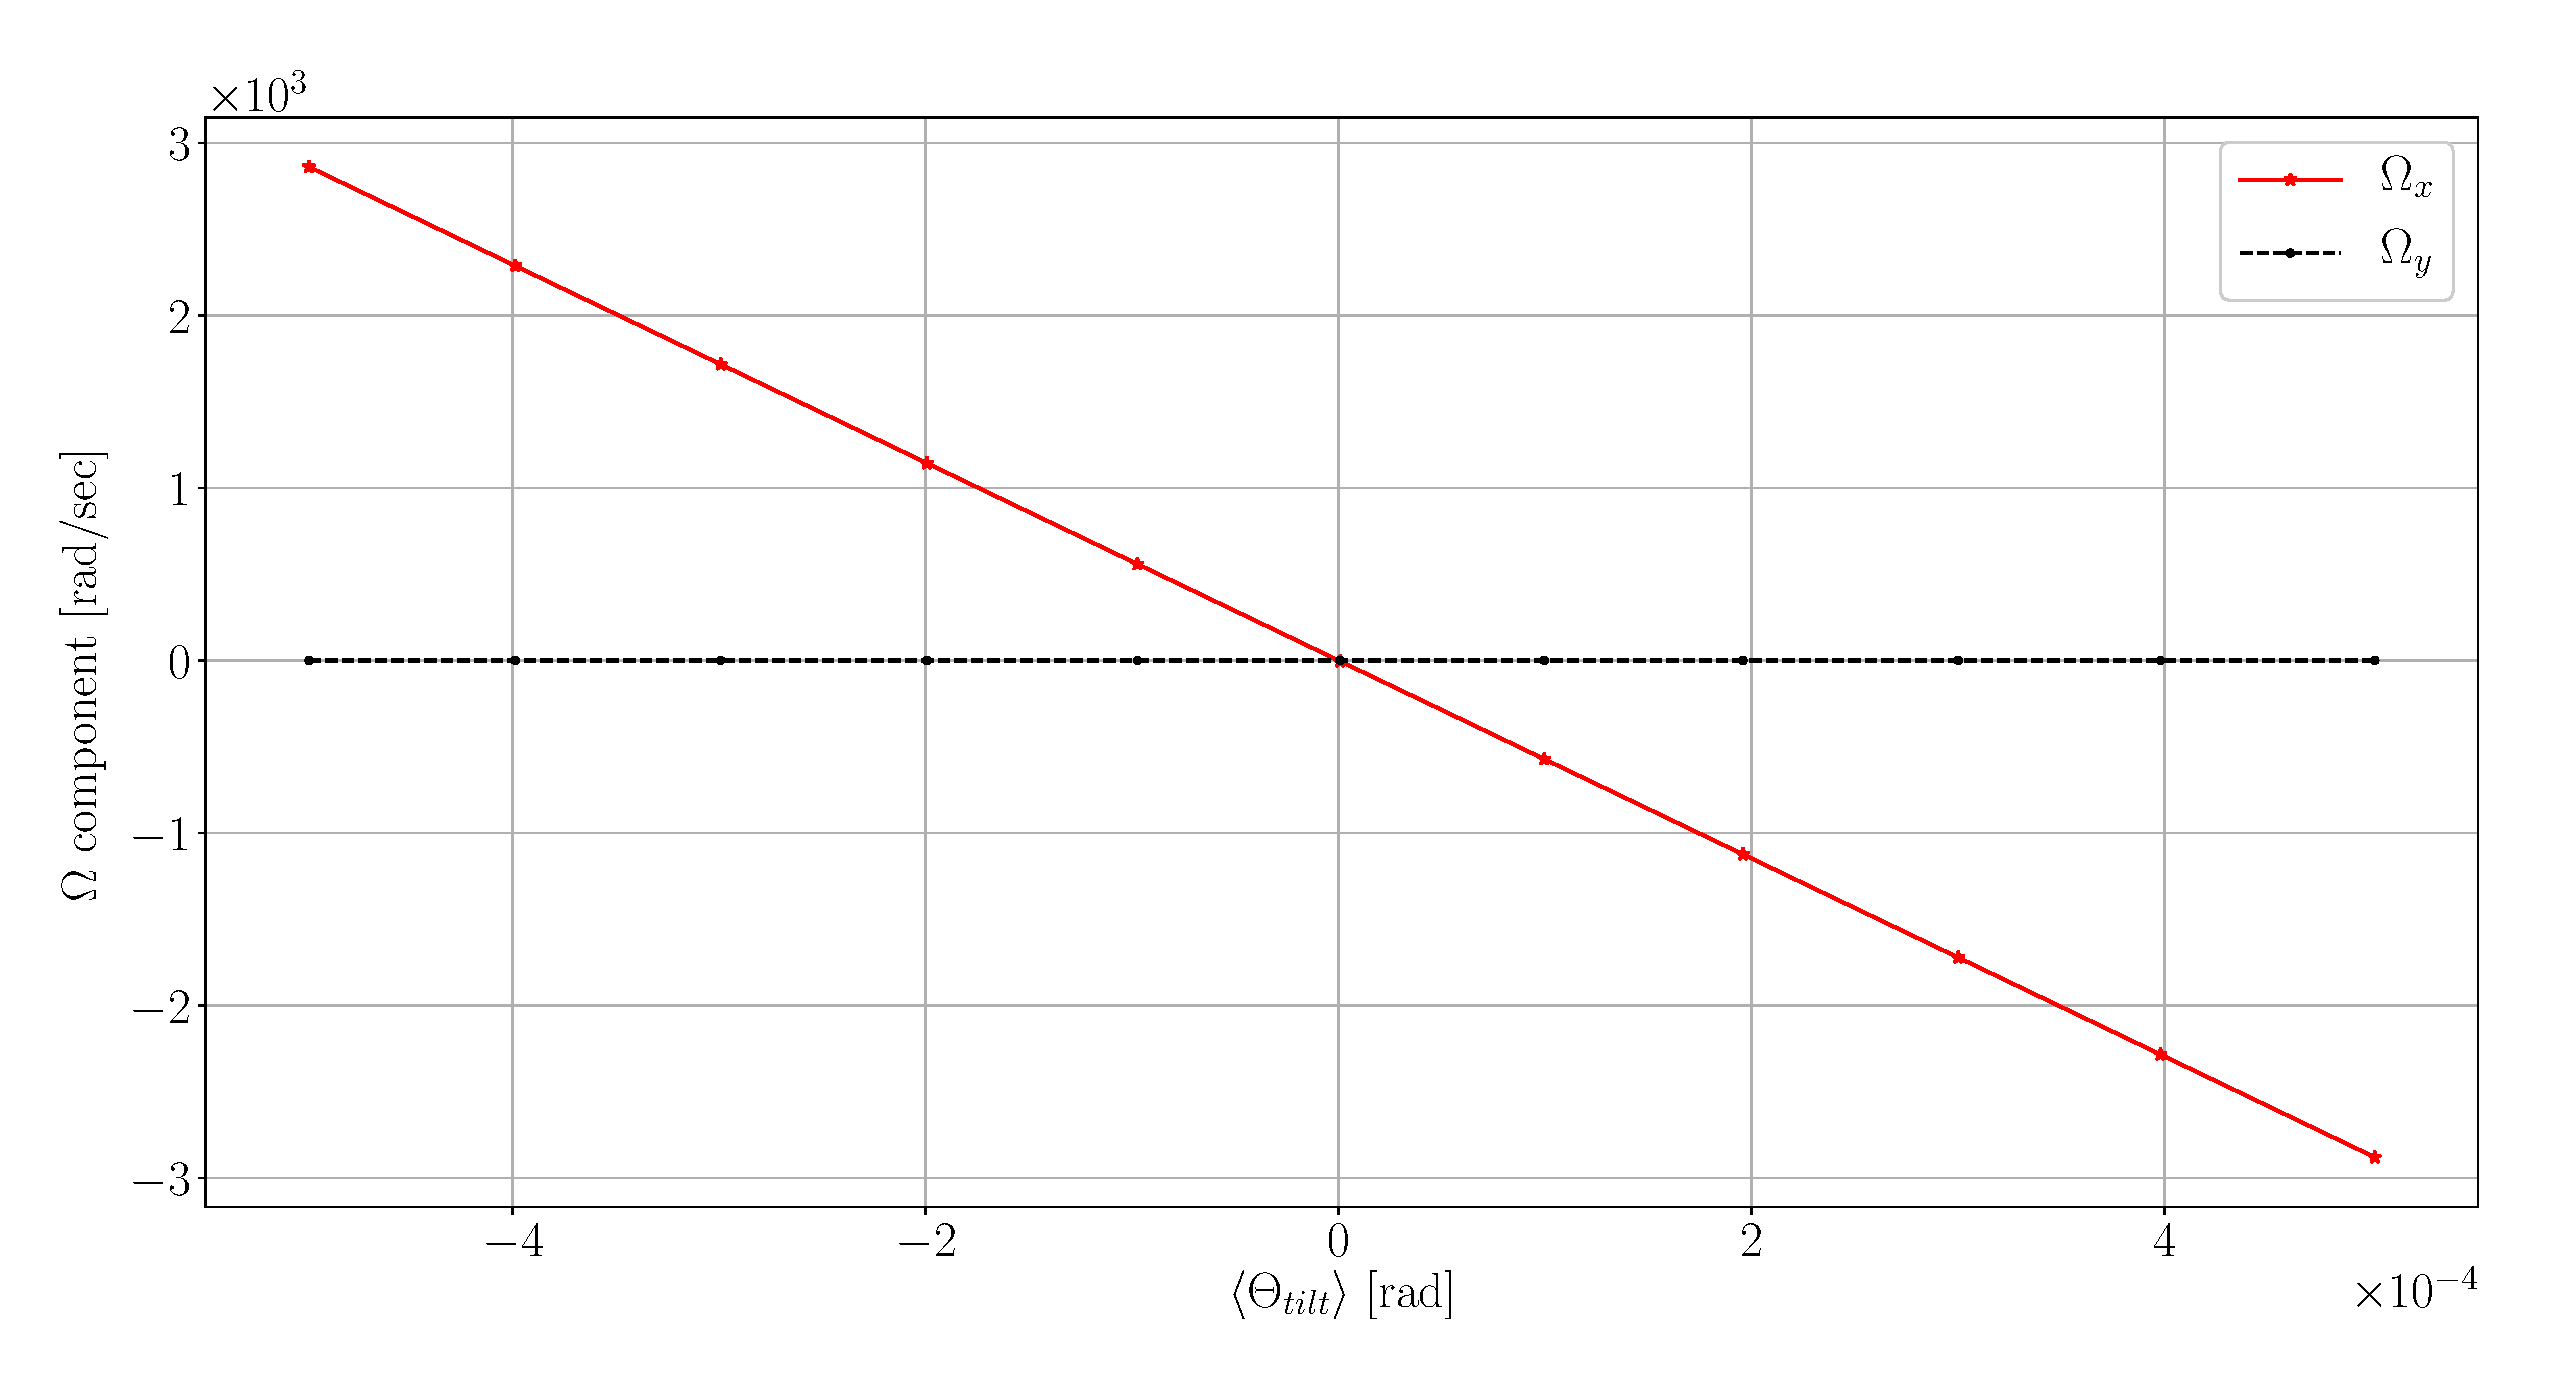
\includegraphics[height=.35\paperheight]{images/fake_signal_sim/linearity_test_shifting_gauss_freq}
		\caption{Angular velocity $\vec\W$ components.}
	\end{subfigure}
	\caption{Reference particle's spin precession axis and angular velocity components as
		 functions of the mean E+B element tilt angle. Element tilts are normally distributed.
		Color identifies the component; radial (blue) and vertical (orange).\label{fig:Linearity_test_shifting_gauss}}
\end{figure}

One can observe from the figure that a tilt distribution at which the mean tilt angle is equal to $10^{-4}$ radians, the
beam polarization vector precesses in the vertical plane at the rate of 500 rad/sec. This agrees with the estimates
mentioned above (section~\ref{chpt3:imperfections}), because in them a tilt error standard deviation of $10^{-4}$ rad 
is assumed at 100 tilted elements. In that case, the mean tilt angle standard deviation is $10^{-5}$, and hence MDM
precession occurs at a rate up to 50 rad/sec with a probability 67\%, and up to 100 rad/sec with a probability 95\%.

Figure~\ref{fig:Linearity_test_compensated} shows the results of a simulation in which six randomly-picked
E+B elements were pair-wise tilted by opposite angles, while one element was tilted by an angle
$\mu_i = (i-5)\cdot 10^{-6}$ rad, $i\in\lbrace0,\dots,10\rbrace$. 

Both simulations were done at the strict FS energy 270.0092 MeV.\footnote{At this energy, in the ideal lattice, 
	$\nu_s$ and $\nbar$	are undefined in the beam rest frame used in COSY Infinity.
	This corresponds to the situation when spin does not precess in any plane (either horizontal or vertical), 
	which corresponds to the realization of the 3D FS condition in an ideal lattice.} One can see that the compensated
elements do not contribute to the spin precession.

\begin{figure}[!h]
	\centering
	\begin{subfigure}{\linewidth}
		\includegraphics[height=.35\paperheight]{images/fake_signal_sim/linearity_test_compensated+microrad_nbar}
		\caption{Spin precession axis $\nbar$ components.}
	\end{subfigure}
	\begin{subfigure}{\linewidth}
		\includegraphics[height=.35\paperheight]{images/fake_signal_sim/linearity_test_compensated+microrad_freq}
		\caption{Angular velocity vector $\vec\W$ components.}
	\end{subfigure}
	\caption{Reference particle's spin precession axis and angular velocity components as
		functions of the mean E+B element tilt angle. Three mutually-compensated tilt pairs plus an uncompensated
		rotation.
		Color identifies the component; radial (blue) and vertical (orange)\label{fig:Linearity_test_compensated}}
\end{figure}

\subsection{Comparison of the CW vs CCW beams' spin precession angular velocities}\label{chpt3:imperfections:CW_vs_CCW}
In Figure~\ref{fig:Lin_test_rel_diff} we plotted the relative difference between the CW and CCW beams' radial SPA/angular velocity
components in the case of both the normally-distributed and mutually-compensated tilt cases.

For the raidal SPA component the relative difference was computed as
\[
\delta\bar n_x = \frac{\bar n_x^{CW}(\avg{\Theta_{tilt}}) - \bar n_x^{CCW}(\avg{\Theta_{tilt}})}{\bar n_x^{CW}(\avg{\Theta_{tilt}})};
\]
for the angular velocity:
\[
\delta\W_x = \frac{\W_x^{CW}(\avg{\Theta_{tilt}}) - \W_x^{CCW}(\avg{\Theta_{tilt}})}{\W_x^{CW}(\avg{\Theta_{tilt}})}.
\]

In the figures, one can observe that in either case both beams' SPA is oriented the same way; 
there is some difference between the beams' spin tunes, but it stays below the percent level. 
The spin tune difference grows bigger as the
spin wheel roll rate (proportional to the mean tilt angle) gets slower. 
The spin tune difference may indicate that
the lattice is asymmetric, with respect to the spin dynamics, relative to the beam circulation direction (i.e. time reversal).
It may be explained by a difference between the CW and CCW beams' closed orbits.

\begin{figure}[!h]
	\centering
	\begin{subfigure}{\linewidth}
		\includegraphics[height=.35\paperheight]{images/fake_signal_sim/linearity_test_shifting_gauss_rel_diff}	
		\caption{Normally distributed E+B element tilts.}
	\end{subfigure}
	\begin{subfigure}{\linewidth}
		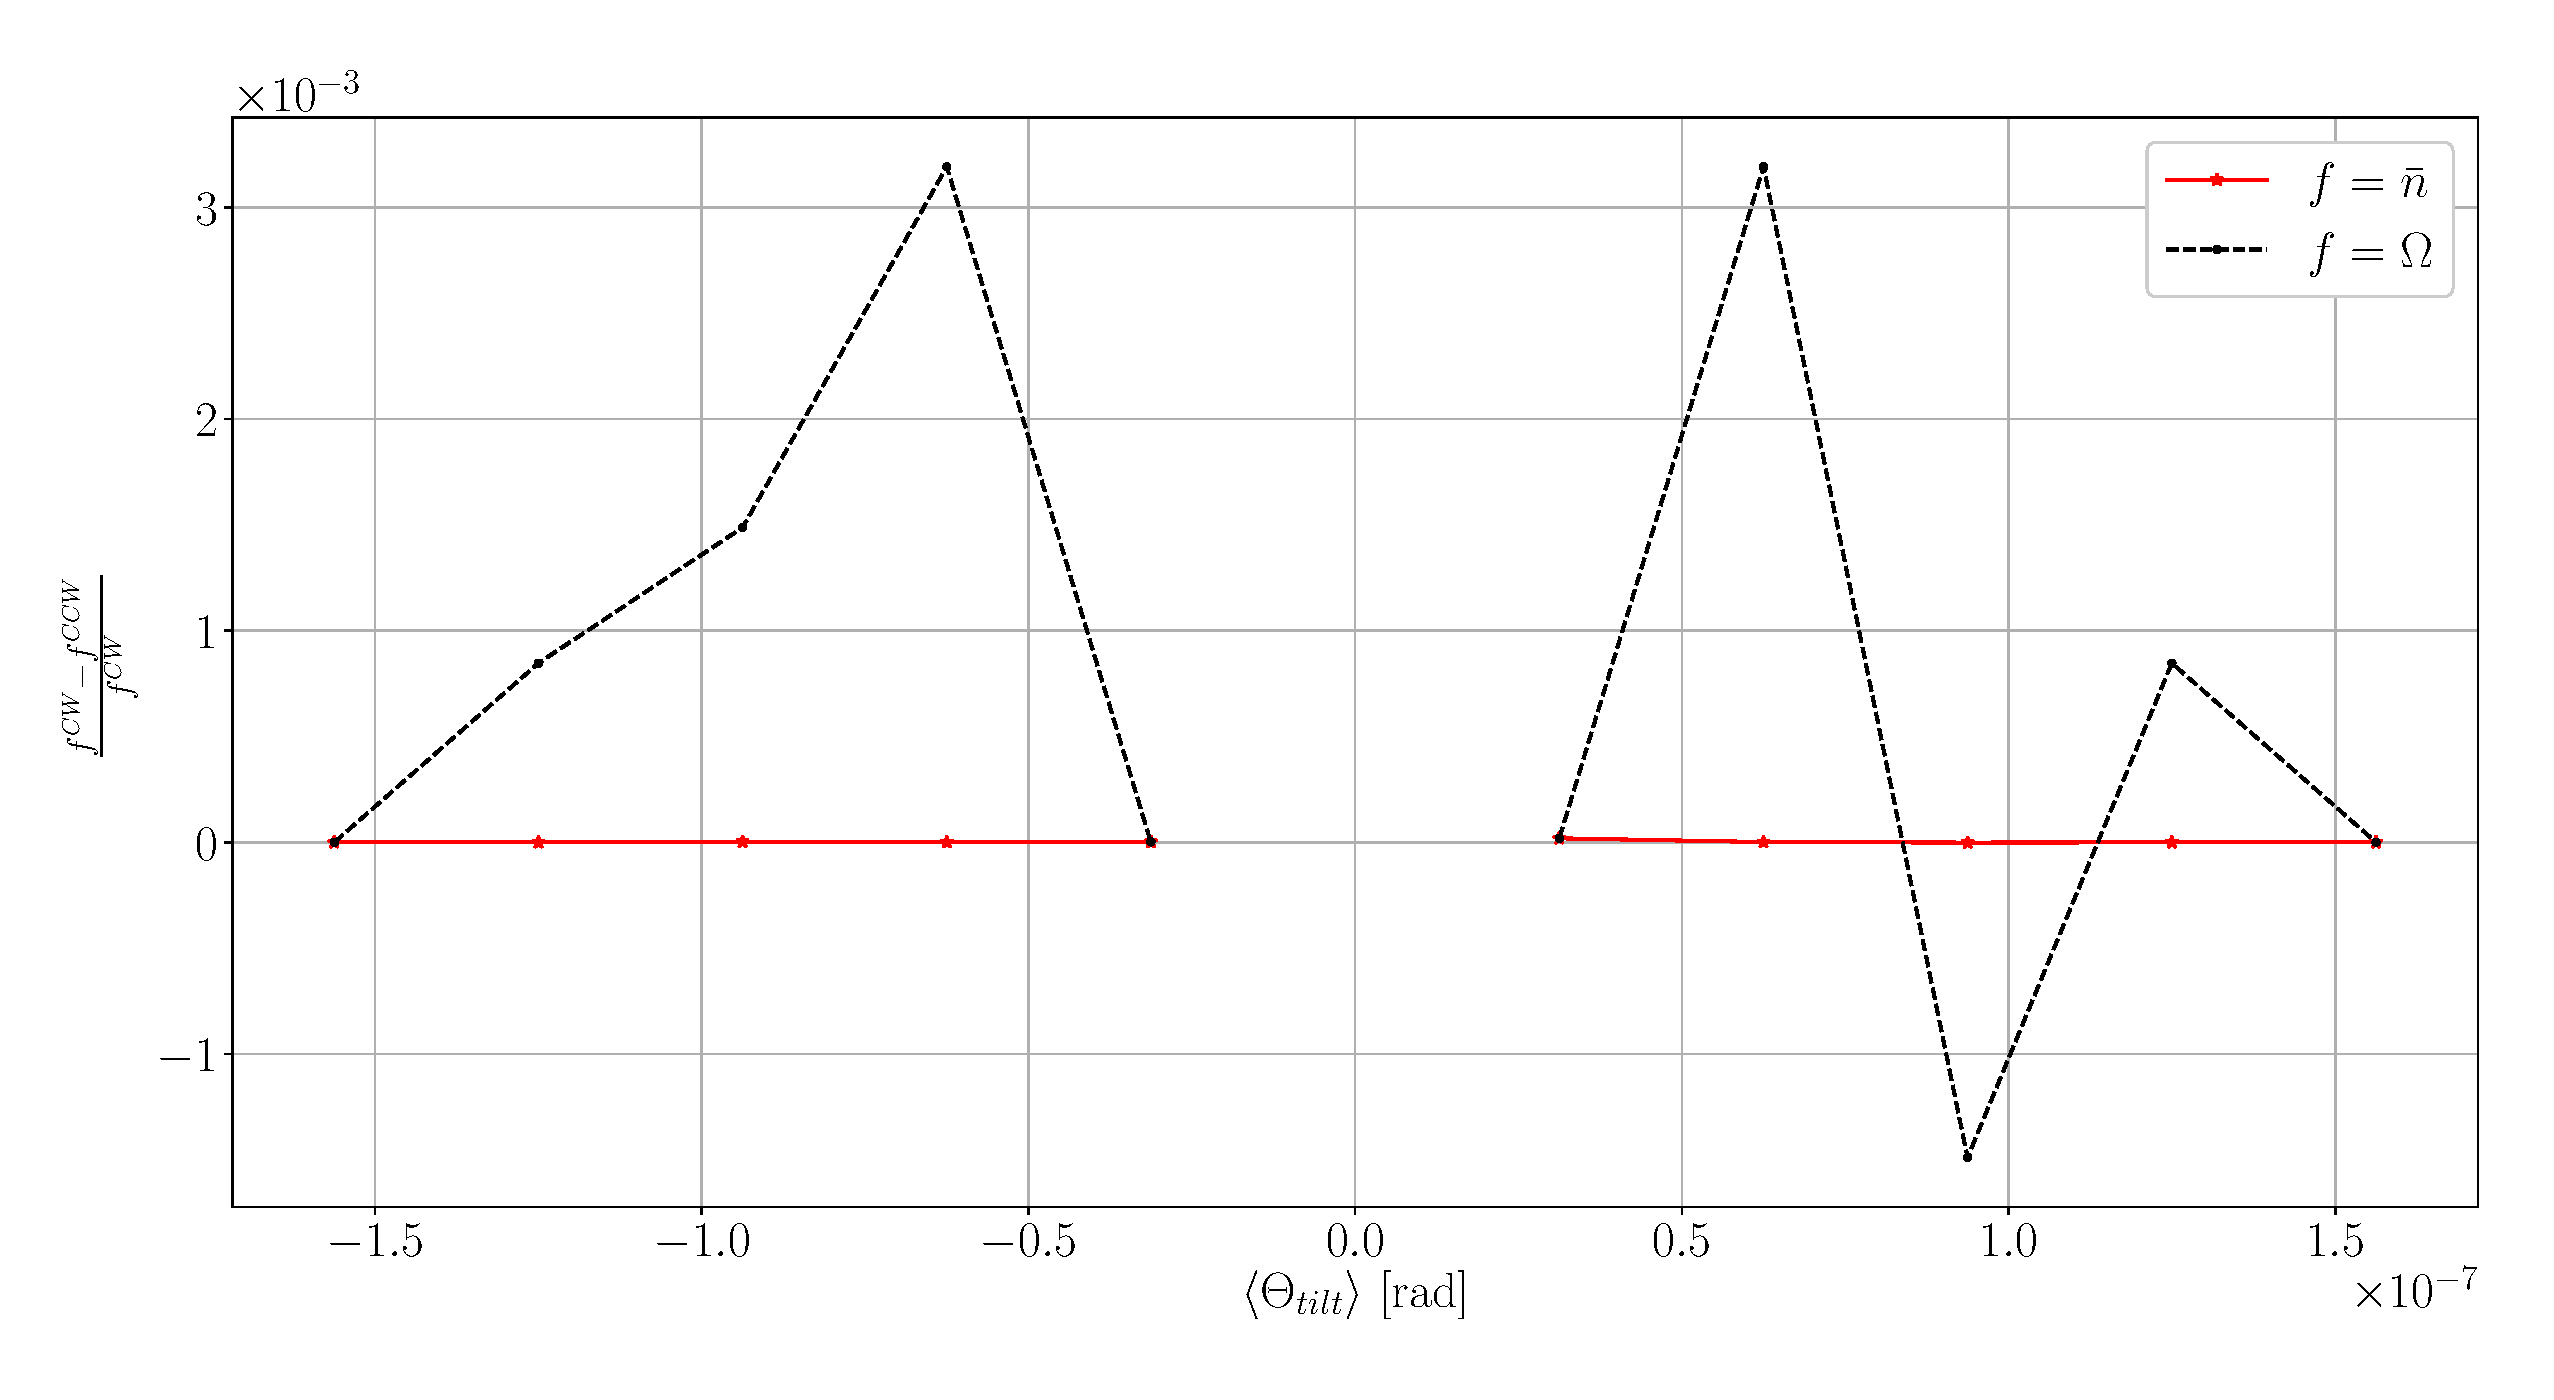
\includegraphics[height=.35\paperheight]{images/fake_signal_sim/linearity_test_compensated+microrad_rel_diff}
		\caption{Mutually-compensated element tilts.}
	\end{subfigure}
	\caption{Relative difference between the CW and CCW beams' spin precession axis and angular velocity radial components.
		Color marks the compared variable: spin precession axis (blue) and abgular velocity (orange).\label{fig:Lin_test_rel_diff}}
\end{figure}


\section{Смена полярности ведущего поля}\label{chpt3:GFF}
%Смена полярности ведущего магнитного поля комбинированного накопительного кольца производится для того, чтобы инжектировать пучок в обратном направлении. При этом, величина $E_r = \frac{GB_yc\beta\gamma^2}{1-G\beta^2\gamma^2}$ электростатического поля (см. раздел~\ref{sec:FS_in_a_ring}) остаётся фиксированной. Так делается для сохранения величины и направления $\vec\w_x^{EDM}$. Наша задача, при смене полярности поля --- гарантировать равенство по модулю, и противоположность по направлению, векторов $\vec\w^{MDM,CW}$ и $\vec\w^{MDM, CCW}$.

Необходимо уделить внимание двум аспектам проблемы смены полярности ведушего поля:
\begin{enumerate}
	\item Какой параметр системы должен оставаться постоянным от цикла к циклу;
	\item Как его можно наблюдать.
\end{enumerate}

Целью смены полярности ведущего поля является точное воспроизведение радиальной компоненты
частоты МДМ прецессии, индуцированной полями неидеальности ускорителя. Этот момент часто упускается из виду:
простое воспроизведение \emph{величины магнитного поля} не достаточно, поскольку точка инжекции центроида пучка,
а значит его длина орбиты --- и соответственно, ввиду уравнений~\eqref{eq:EffectiveGamma}
 и~\eqref{eq:spin_tune_vs_gamma}, спин-тюн, --- подвержена вариации. (Помимо этого, ускорительная структура
  может быть асимметрична,	с точки зрения спиновой динамики, относительно обращения 
  направления движения пучка.)

Таким образом, необходимо восстанавливать не величину поля, а эффективный Лоренц-фактор центроида.

Касательно второго вопроса, мы уже говорили, что скорость вращения Спин-Колеса
контролируется через измерения частоты прецессии спина в горизонтальной плоскости. 
Эта плоскость была выбрана потому, что вектор угловой скорости ЭДМ прецессии смотрит
(по большей части) в радиальном направлении; его вертикальная компонента возникает из-за полей
неидеальности ускорителя, и мала по-сравнению с ихмеряемым ЭДМ эффектом.
Поэтому, в первом приближении, когда мы манипулируем вертикальной компонентой совокупной угловой скорости спин-прецессии, мы манипулируем вертикальной компонентой вектора угловой скорости МДМ-прецессии.

Процедура калибровки эффективного Лоренц-фактора состоит в следующем.

\documentclass{article}

\usepackage{phdstyle}
\usepackage[numbers]{natbib}



\begin{document}

Problem statement. Effective gamma concept. Calibration of the magnetic field by the horizontal precession frequency. Simulation results.
\newpage


In the FD method, the misalignment-caused MDM precession is dealt with by adding up spin precession frequencies, one of which is measured when the beam is revolving in the storage ring clockwise, the other counter-clockwise (eq~\eqref{eq:FDM_estimator}). This is problematic for two reasons:
\begin{enumerate}
\item In order to change the beam revolution direction, the guiding magnetic field needs to be flipped. The problem is to reproduce the field strength; currently, no direct magnetic field measurement methods provide sufficient precision.
\item The two beam orbits will most certainly be different, potentially being a source of error.
\end{enumerate}

The second point was addressed in section~\ref{sec:Decoh_origin}, when we introduced the concept of the effective Lorentz factor. The spin tunes of particles characterized by the same $\gamma_{eff}$ are equal, even if their orbital dynamics are completely different. Since frequencies alone are involved in the determination of the EDM effect, the FD methodology is insensitive to variation in the beam dynamics.


We note that the FS condition for the deuteron is realized by a combination of the electric and magnetic field strengths, and the beam energy. Also, the electric field configuration need not be changed when changing the beam revolution direction. Therefore, for any beam injection energy there exists one, and only one, guide field strength, at which the FS condition is realized (in the horizontal plane).

This fact is used in the FD methodology. The argument runs as follows:
\begin{itemize}
\item assuming the EDM precession about the y-axis is negligible;
  \item $\W_y^{MDM}\propto B_y$, $W_x^{MDM}\propto B_x$, and $\frac{B_x}{B_y} = \tan\theta$, where $\theta$ is the rotation angle of the element about the optic axis $s$ (tilt), caused by magnet misalignment;
\item when we reverse the direction of the field, the relationship between $B_y$ and $B_x$ is preserved;
\item therefore, if $\W_y^{MDM, CCW} = -\W_y^{MDM, CW}$, then $B_y^{CCW} = -B_y^{CW}$, then $B_x^{CCW} = -B_x^{CW}$, and therefore, $\W_x^{MDM, CCW} = -\W_x^{MDM, CW}$.
\end{itemize}
That is, once 

We gain the following advantages: 


\end{document}


\section{Спин-тюн эквивалентность траекторий частиц с одинаковыми значениями эффективного Лоренц-фактора}\label{sec:spin_tune_traj_equivalence}
В контексте процедуры смены направления вращения Спин-Колеса, важно рассмотреть вопрос эквивалентности спин-динамики CW и CCW пучков. 

Отправной точкой нашего анализа является утверждение 1: частицы с одинаковым значением эффективного Лоренц-фактора имеют одинаковый спин-тюн, то есть эквивалентны с точки зрения спиновой динамики. Это следствие уравнения~\eqref{eq:spin_tune_vs_gamma}.

В следующих разделах мы проанализируем две формулировки утверждения 1:
\begin{enumerate}[A.]
	\item интерпретируя эффективный Лоренц-фактор как математическое ожидание кинетической энергии частицы;
	\item функция многих переменных $\nu_s(x, a, y, b, \ell, \delta)$ агностична к фазовой траектории частицы в поперечном фазовом пространстве $(x,a)$, и $(y,b)$, т.е. может быть сведена к функции одной переменной $\nu_s(\g*)$.
\end{enumerate}

\subsection{Формулировка A}

In this section we will consider Statement 1, interpreting the effective Lorentz factor as the expectation value
of a particle's Lorentz factor.

In order to test this formulation we carried our the following simulation: we injected three 10-particle
bunches (X, Y, and D) into the ideal FS lattice. The orbital and spin transfer matrices were computed
up to the third-order Taylor expansion; the particle injection energy was 270 MeV. The X-bunch particles
were uniformly distributed along the radial axis in the range $\pm 1$ mm; those of the Y-bunch, along the vertical
axis in the range $\pm 1.318$ mm;~\footnote{This range was chosen in order to equalize the transverse
emittances of the particles. The initial coordinate offset determines the betatron oscillation amplitude $A$,
which is related to the beta function $\beta$ and transverse emittance $\epsilon$ as in
$A = \sqrt{\epsilon \beta}$.} the D-bunch particles were distributed by $\Delta K/K_0$ in the range $\pm 10^{-4}$.
Then spin tracking was done for 12,000 turns, with data recorded every 80 turns.

The recorded data were: the particle phase space coordinate $\vec z = (x,x',y,y',\ell, \delta)$, where
$\ell = -(t-t_0)v_0\frac{\gamma_0}{1+\gamma_0}$ is the particle's longitudinal offset relative to the
reference partilce, $\delta = \Delta K/K$ is its energy offset, as well as its spin tune $\nu_s(\vec z)$.
Based on these data we computed the particles' time-average spin tune $\avg{\nu_s}$,
energy offset  $\avg{\Delta K/K}$, and longitudinal and transverse emittances.

In Figure~\ref{fig:stune_traj_equ_main} are presented the simulation results. On the top panel is plotted the
dependence of $\avg{\nu_s}$ on $\avg{\Delta K/K}$ for the betatron-oscillating bunches when the sextupoles
are turned off. One can see from the figure that, at the same mean energy level, the particles betatron
oscillating in the horizontal plane have spin tune different from that of the vertical plane betatron
oscillating particles. This means, as far as we can tell, that Statement 1 in formulation A is disproven.

We hypothesized that the difference in the plotted lines' slopes is related to the
\emph{spatial dependence} of the momentum compaction factor.

This hypothesis is based on our analysis of the sextupole field suppression effects' signatures, described
in detail in section~\ref{sec:sext_decoh_suppression_effect_analysis}. In order to test this hypothesis we
repeated the experiment at different values of the GSX sextupole gradient, taken from
the range $\pm 5\cdot 10^{-3}$. The simulation results are shown in Figure~\ref{fig:stune_traj_equ_main}.
The same dependence is plotted as previously, but only for the X-bunch.
As one can see, when the gradient is varied the slope varies with it. The same behavior as was
observed in section~\ref{sec:sext_decoh_suppression_effect_analysis}.

\begin{figure}[h]
	\centering
	\includegraphics[height=.3\paperheight]{images/stune_traj_equ/part1/stune_vs_equ_energy}
	\caption[Mean spin tune level veresus mean kinetic energy level.]{Particle mean spin tune level
        as a function of its mean kinetic energy level. Top panel: sextupoles are off for both injected bunches.
        Bottom panel: X-bunch dependencies at different GSX gradients.\label{fig:stune_traj_equ_main}}
\end{figure}

In order to check the hypothesis about the spatial dependence of the momentum compaction factor we computed
the dependencies of the mean energy levels of the X- and Y-bunch particles on their betatron tune-normalized
transverse emittances (Fiugre~\ref{fig:equ_nrg_vs_emittance}).
According to equation~\eqref{eq:betatron_OL}, the orbit lengthening of particles with equal Q-normalized
transverse emittances must be equal. The equilibrium energy level shift of a particle is proportional to
its orbil lengthening via the momentum compaction factor; hence the slope difference seen in
Figure~\ref{fig:equ_nrg_vs_emittance} is evidence that the momentum compaction factors experienced by the
X-, and Y-bunches are different. 

\begin{figure}[h]
	\centering
	\includegraphics[height=.3\paperheight]{images/stune_traj_equ/part1/equ_energy_vs_emittance}
	\caption{Longitudinal emittance dependence of the mean energy level.\label{fig:equ_nrg_vs_emittance}}
\end{figure}

The observed longitudinal dependence of the momentum compaction factor is further confirmed by equation~(15)
of reference~\cite{Senichev:IPAC13}, in which we find:
\[
\alpha_0 = \avg{\frac{D_0}{\rho}},~~ \alpha_1 = \avg{\frac{D_1}{\rho}} + \frac12\avg{D_0'^2},
\]
where $D(s) = D_0(s) + D_1(s)\cdot \delta$  is the dispersion function, $\rho$ the radius of the clsed orbit.
In first approximation, dispersion exists only in the horizontal plane and is zero in the vertical plane,
meaning that the spatial dependence of the dispersion function reflects on the spatial dependence of the momentum
compaction factor.

For comparison, the same tests were carried out with linear Taylor expansions of the spin and orbital
transfer maps. The results are whoen in Figures~\ref{fig:stune_traj_equ_linear:stune_vs_nrg},
and~\ref{fig:stune_traj_equ_linear:nrg_vs_emittance}. As one can see in
Figure~\ref{fig:stune_traj_equ_linear:nrg_vs_emittance}, all particles doing betatron oscillations in the
vertical plane share the same value of the mean energy level, which is an indication that they share
the same closed orbit, which in turn means there's no dispersion in the vertical plane.
In this case also follows, from Figure~\ref{fig:stune_traj_equ_linear:stune_vs_nrg}, that their spin tunes
are equal.

\begin{figure}[h]
\centering
\begin{subfigure}{\linewidth}
\includegraphics[width=\linewidth]{images/stune_traj_equ/part1/equ_energy_vs_emittance_linear}
\caption{Mean energy level dependence on
particle transverse emittance\label{fig:stune_traj_equ_linear:nrg_vs_emittance}}
\end{subfigure} 
\begin{subfigure}{\linewidth}
\includegraphics[width=\linewidth]{images/stune_traj_equ/part1/stune_vs_equ_energy_linear}
\caption{Mean spin tune dependence on mean energy.\label{fig:stune_traj_equ_linear:stune_vs_nrg}}
\end{subfigure} 
\caption{Simulation results in the case of linear transfer maps.}
\end{figure}

In Figure~\ref{fig:long_emitt_vs_trans_emitt} are plotted the particle longitudinal emittance as a
function of its Q-normalized transverse emittance. As one can see, the transverse emittances induce
the longitudianl emittances at different rates, depending on the betatron oscillation plane.
In the linear case, vertical plane betatron oscillations do not induce synchrotron oscillations at all.
\begin{figure}[h]
\centering
\begin{subfigure}{\linewidth}
\includegraphics[height=.3\paperheight]{images/stune_traj_equ/part1/long_emitt_vs_trans_emitt}
\caption{Non-linear transfer maps.}
\end{subfigure}
\begin{subfigure}{\linewidth}
\includegraphics[height=.3\paperheight]{images/stune_traj_equ/part1/long_emitt_vs_trans_emitt_linear}
\caption{Linear transfer maps.}
\end{subfigure}
\caption{Longitudinal emittance as a function of
Q-normalized transverse emittance.\label{fig:long_emitt_vs_trans_emitt}}
\end{figure}

\paragraph{Conclusion:} formulation A of Statement 1 is false. 


\subsection{Формулировка B}\label{sec:spin_stune_traj_equ:B_form}
\newcommand{\Ps}{\mathcal P}

Usinf COSY Infinity we compute the Taylor expantion of spin tune $\nu_s(\vec z)$, where
\begin{align*}
  \vec z &= (x,a,y,b,\ell,\delta), \\
  \ell &= -(t - t_0)v_0\frac{\gamma-1}{\gamma}, \\
  \delta &= \frac{\Delta K}{K}.
\end{align*}

In the present section we will test formulation B of Statement 1:
the multivariate function $\nu_s(\vec z)$ can be expressed as a function of a single scalar parameter
$\nu_s(\g*)$. We will not assume any formal expression of $\g*$.

If formulation B is correct, there exists a coordinate system (with one axis being $\nu_s$),
in which horizontal plane betatron oscillating particles are indistinguishable, in terms of spin tune,
from vertical plane betatron oscillating particles. This coordinate system, hence, must not include
coordinates from the transverse phase space planes $(x,a)$, and $(y,b)$.

Therefore, we will look at the space $\Ps=(\ell, \delta, \nu_s)$. If formulation B is correct,
differences between particles' transverse phase plane trajectories must not reflect on their
trajetctories in $\Ps$.

We used the same data in this analysis as in the previous section.

In Figure~\ref{fig:main:all_ps} $\nu_s(\vec z)$ is plotted as a function of $(\ell, \delta)$ when
$\vec z$ is the real trajectory the particle takes in the storage ring. We observe:
\begin{enumerate}
\item the same stratification of the mean spin tune levels as in section~\ref{sec:decoh:sim-imperfect};
  \item the stratification if more pronounced for the X-bunch (blue dots), than for the Y-bunch (red dots).
\end{enumerate}

The latter can be explained by thee greater magnitude of the dispersion function in the horizontal plane.
Note that at equal values of the Q-normalized transverse emittance~\footnote{Q-normalized is $\epsilon_\alpha\cdot Q_\alpha$, where $\alpha\in\{x,y\}$.} (i.e. at equal orbit lengthenings, if equation~\eqref{eq:betatron_OL}
is to be believed), horizontal plane betatron oscillating particles have a greater longitudinal emittance than
those oscillating in the vertical plane.

\begin{figure}[h]
  \centering
  \begin{subfigure}{\linewidth}
    \includegraphics[height=.3\paperheight]{images/stune_traj_equ/part2/3D_plot_all_ps_vars}
    \caption{Particles picked according to the values of their Q-normalized \emph{transverse}
    emittances.\label{fig:main:all_ps}}
  \end{subfigure}
  \begin{subfigure}{\linewidth}
    \includegraphics[height=.3\paperheight]{images/stune_traj_equ/part2/3D_plot_all_ps_vars_equal_long_emi}
    \caption{Particles are picked according to the values of their \emph{longitudinal}
    emittances.\label{fig:main:gamma_eff}}
  \end{subfigure}
  \caption{Spin tune as a function of the particle's position in the longitudinal phase space.
    Colors mark the bunch: blue for X, red for Y. The corresponding Q-normalized transverse and
    longitudinal emittances are shown in the legend.\label{fig:main}}
\end{figure}

Due to the latter fact, we decided to plot the same dependence, but to pick particles based on the equality of
their longitudinal, instead of transverse, emittances. In Figure~\ref{fig:main:gamma_eff} we observe that
particles having similar magnitudes of their longitudinal emittance have also silimar mean spin tune levels.

\paragraph{Conclusion:} formulation B is confirmed by simulation; the effective Lorentz factor reflects the
magnitude of the particle's longitudinal emittance.

In view of Figure~\ref{decoh:fig:nbar_vs_ST}, one can also conclude that particles with equal
effective L-factor values are spin dynamics-equivalent in the general sense, by which we mean that
they have not only equal values of spin tune, but the same orientation of the invariant spin axis.~\footnote{
At any rate, this seems to be true in the FS regime of operation.}


\clearpage
